\documentclass[journal=jpcbfk,manuscript=article]{achemso}

\usepackage{graphicx}
\usepackage{wrapfig}
\usepackage{subcaption}
\usepackage{amsmath} % or simply amstext
\usepackage{amssymb}
\usepackage{siunitx}
\usepackage{booktabs}
\usepackage[export]{adjustbox}
\newcommand{\angstrom}{\textup{\AA}}
\usepackage{cleveref}
\usepackage{booktabs}
\usepackage{gensymb}
\usepackage{float}
\usepackage{xr}
\usepackage{enumitem}
\newcommand{\nclusters}{10}
%\DeclareUnicodeCharacter{03C9}{$\omega$}
\externaldocument[S-]{Supporting_Information}

\SectionNumbersOn

\title{Statistical Inference of Transport Mechanisms and Long Time Scale Behavior from Time Series 
       of Solute Trajectories in Nanostructured Membranes}
\author{Benjamin J. Coscia}
\affiliation{Department of Chemical and Biological Engineering, University of Colorado Boulder, Boulder, CO 80309, USA}
\author{Christopher P. Calderon}
\affiliation{Department of Chemical and Biological Engineering, University of Colorado Boulder, Boulder, CO 80309, USA}
\author{Michael R. Shirts}
\email{michael.shirts@colorado.edu}
\affiliation{Department of Chemical and Biological Engineering, University of Colorado Boulder, Boulder, CO 80309, USA}

\begin{document}

  \graphicspath{{./figures/}}
  \maketitle
  
  \begin{abstract}

  Appropriate time series modeling of complex diffusion in soft matter systems on the
  microsecond time scale can provide a path towards inferring transport mechanisms and
  predicting bulk properties characteristic of much longer time scales. In this work 
  we apply the infinite hidden Markov model (IHMM) to solute center-of-mass trajectories
  generated from long molecular dynamics simulations in a cross-linked inverted hexagonal
  phase lyotropic liquid crystal (LLC) membrane in order to automatically detect a
  variety of solute dynamical states which can be further explained in terms of 
  solute-membrane interactions.

  We group the states identified by the IHMM into clusters based on multiple metrics
  aimed at distinguishing solute behavior based on their fluctuations, dwell times
  in each state and position within the inhomogeneous membrane structure. We analyze
  prevalent clusters in order to relate their parameters to physical interactions between 
  solutes and the membrane. 

  Along with parameters of individual states, the IHMM simultaneously infers a transition
  matrix which allows us to stochastically propagate solute behavior from all of the 
  independent trajectories onto much longer time scales while still preserving the 
  qualitative behavior characteristic of the MD trajectories. This affords a direct 
  connection to important macroscopic observables used to characterize performance like
  solute flux and selectivity. 
  
  Overall, this work provides an effective way to simultaneously identify transport 
  mechanisms in nanoporous materials and project complex diffusive behavior on
  long time scales.  This enhancement to our understanding of the diverse range 
  of solute behavior allows us to hypothesize design changes 
  to LLC monomers aimed towards controlling the rates of solute passage, thus improving 
  the selective performance of LLC membranes. 
  
  \end{abstract}  
  
  
  \section{Introduction}
  
  There is a need for highly selective membranes in order to perform efficient 
  separations of the components of complex aqueous streams.
  \begin{itemize}
    \item Desalination and boric acid removal from seawater.
    \item Organic micropollutants
    \item Hydraulic fracturing flowback water
    \item Breathable chemical warfare agent barriers
    \item High purity chemicals
    \item While many researchers focus on membrane permeability, we may be 
    able to reduce costs of commercial nanofiltration and reverse osmosis with
    higher selectivity.~\cite{werber_materials_2016}
  \end{itemize}
  
  The ability to efficiently design novel membrane materials for selective separations
  would be greatly enhanced by easily interpretable methods for connecting microscopic
  fluctuations with macroscopic observables. If one could apply molecular dynamics 
  (MD) simulations to explain important experimental metrics such as solute flux and 
  selectivity in terms of detailed chemically dependent solute motion, then we can more
  easily bridge the disconnect between theory and application. In many systems, it's 
  possible to achieve this by calculating diffusion constants. Unfortunately, for 
  systems which exhibit complex short timescale subdiffusive dynamics, one cannot 
  calculate reliable diffusion constants since solute mean square displacements (MSDs)
  are non-linear on the timescales accessible to molecular simulation. Therefore, we
  are in need of a more flexible approach for modeling solute dynamics which makes 
  less assumptions about the solute's average behavior.
  
  In this work, we are particularly interested in the design of lyotropic liquid crystal (LLC)
  monomers, a class of amphiphilic molecules whose ordered self-assembled phases can be 
  cross-linked into mechanically strong membranes capable of highly selective separations.
  \begin{itemize}
  	\item Inverted hexagonal, H\textsubscript{II}, phase LLC membranes are characterized
  	by hexagonally packed, uniform-sized and straight pores, an ideal geometry for high 
  	throughput transport.
	\item Their pores are lined with the LLC monomer functional groups which can
	potentially be designed to interact with solutes in a chemically-specific manner.
	\item It would be extremely useful to experimentalists if we could connect LLC monomer
	design with measurable quantities.
	\item This goal is complicated by the non-Brownian hopping and trapping behavior induced
	by the membrane's diverse topology and inhomogeneous structure.~\cite{coscia_understanding_2019,coscia_chemically_2019}
  \end{itemize}
  
  We have already progressed our understanding of LLC monomer design in our previous work
  by building stochastic time series models based on the chemical intuition gained
  from qualitative MD studies of solute transport in an H\textsubscript{II} phase LLC
  membrane.~\cite{coscia_chemically_2019,coscia_capturing_2020}
  \begin{itemize}
    \item We identified three classes of trapping behavior which result in short time scale
    subdiffusion.
    \item In our first approach to stochastically model this behavior, we treated the
    system's dynamics as a sequence of anti-correlated hops between power law distributed
    periods of entrapment, a framework called subordinated fractional Brownian or L\'evy
    motion.
    \item In a second approach, we treated solute motion as a Markov state model with 
    state-dependent dynamics, where we parameterized the state transition probabilities 
    between each of eight discrete states, defined by the observed trapping mechanism, 
    as well as the solute dynamics within each of these states. 
    \item We showed how one could use realizations of any stochastic model like these in
    order to predict macroscopic flux and selectivity. 
  \end{itemize}
  
  Although powerful and insightful, our previous work required considerable human effort
  in order to analyze the MD trajectories and to hypothesize stochastic models which
  matched the behavior of solutes.
  \begin{itemize}
    \item It would be significantly more useful and broadly applicable if we could 
    design an approach which automatically distinguishes and parameterizes varied solute 
    dynamics and leaves a facile way to generate an ensemble of stochastic trajectory
    realizations that can be used to predict macroscopic transport properties.
  \end{itemize}
  
  In this work we attempt to minimize human effort by applying the infinite hidden 
  Markov Model (IHMM)~\cite{beal_infinite_2002,calderon_inferring_2015}, a nonparameteric 
  Bayesian classification technique, in order to automatically detect and infer the 
  parameters of an unknown number of latent vector autoregressive (VAR) modes present 
  in solute center-of-mass time series trajectories. 
  \begin{itemize}
    %MRS: start with where it has been used before (to establish utility) a
    \item It's been used extensively for speaker diarization and has found some application
    in single particle trajectory analysis.~\cite{calderon_inferring_2015,fox_sticky_2011}
    %MRS: Then say it hasn't been used in this context (do we know of any, then cite, if none we have found, say so.)
    \item The IHMM has not been used much for MD trajectory analysis.
  \end{itemize}
  
  We aim to address two primary scientific questions with this work:
  First, we want to know whether it is possible to predict macroscopic transport
  properties. We use the VAR parameters and state transition probability matrix of
  the IHMM in order to generate stochastic trajectory realizations with behavior 
  similar to that exhibited by MD. One can project these realizations onto much 
  longer timescales with computational ease extending into timescales where 
  regular diffusive behavior again occurs.
  Second, we want to know if the IHMM algorithm can help researchers
  efficiently uncover underlying transport mechanisms which give rise to different 
  solute dynamical behavior.
  We use the parameters of the states identified by the IHMM in order to infer 
  dominant solute-membrane interactions and transport mechanisms. We cluster similar 
  state parameters in order to reduce the state space and to understand which segments 
  of the solute trajectories exhibit similar behavior. We support our mechanistic 
  hypotheses via quantitative comparison to various physical membrane properties and
  solute-membrane interactions.
  
  \section{Methods}
    
  We ran all MD simulations and energy minimizations using GROMACS 2018.
  ~\cite{bekker_gromacs:_1993,berendsen_gromacs:_1995,van_der_spoel_gromacs:_2005,hess_gromacs_2008}  
  Our python implementation of the IHMM algorithm is available online at \\
  \texttt{https://github.com/bencoscia/hdphmm}. All other post-simulation 
  trajectory analysis tools are available online at
  \texttt{https://github.com/shirtsgroup/LLC\_Membranes}.

  \subsection{Molecular Dynamics Simulations}

  We studied transport of solutes in the H\textsubscript{II} phase using an
  atomistic molecular model of four pores in a monoclinic unit cell with 
  10 \% water by weight. Approximately one third of the water molecules 
  occupy the tail region with the rest near the pore center.
  
  We chose to study a subset of 4 of the fastest moving solutes from our previous
  work: methanol, acetic acid, urea and ethylene glycol.
  In addition to exploring membrane structural space the most, these solutes have a
  relatively diverse set of chemical functionality. For each solute we created a 
  separate system and to 
  each system we added 6 solutes per pore for a total of 24 solutes. This number 
  of solutes per pore provides a balance of a low degree of interaction between 
  solutes and a sufficient amount of data from which to generate statistics on the
  time scales which we simulate. Further details on the setup and equilibration of
  these systems are detailed in our previous work.\cite{coscia_chemically_2019}
  
  We let each solute undergo 5 $\mu$s of MD simulation. We used a time step of 2 fs
  at a pressure of 1 bar and temperature of 300K controlled by the Parrinello-Rahman 
  barostat~\cite{parrinello_polymorphic_1981} and velocity rescale 
  thermostat~\cite{bussi_canonical_2007} respectively. We recorded configurations every 0.5 ns.

  \subsection{The Infinite State Hidden Markov Model}\label{method:IHMM}

  %BJC2: I left section numbers off
  \subsubsection*{Extending Hidden Markov Modeling to an Unknown Number of States}
  
  Hidden Markov models (HMMs) are a useful and widely used technique for modeling
  sequences of observations where the probability of the next observation in a 
  sequence depends, at least in part, on a previous unobserved, latent or hidden,
  state.~\cite{beal_infinite_2002} In the context of our simulations, the observations
  correspond to the center of mass coordinates of the solutes versus time, and the
  states correspond to segments of the trajectory with similar dynamical behavior 
  which gives rise to those types of observations. The probability of transitioning 
  to a state based on the current state is defined in terms of an $n\times n$ 
  transition probability matrix, $T$, where $n$ is the number of states. Unfortunately,
  standard HMMs require $n$ to be known \textit{a priori}. One can partially overcome
  this by testing a range of numbers of hidden states and determining which is the
  best representation of the data.~\cite{pohle_selecting_2017}
  
  The infinite-state HMM overcomes this drawback by placing a hierarchical
  Dirichlet process (HDP) prior on the transition probabilities.~\cite{fox_bayesian_2010} Using some 
  base probability distribution, $H$, a Dirichlet process (DP) generates discrete 
  distributions, $G_0$, over a countably infinite number of probability measures:
  \begin{equation}
      G_0 = \sum_{k=1}^{\infty} \beta_k \delta_{\theta_k} ~~ \theta_k \sim H, \beta \sim GEM(\gamma)
  \end{equation}
  where the $\theta_k$ are values drawn from the base distribution and the weights
  $\beta_k$ come from a stick-breaking process parameterized by the concentration 
  parameter $\gamma$ (equivalently referred to as GEM($\gamma$)).~\cite{halmos_random_1944} In shorthand, this
  specification can be expressed as $G_0 \sim DP(\gamma, H)$. The concentration 
  parameter, $\gamma$, expresses one's confidence in the base distribution $H$.
  We use a uniform base distribution for $H$. When $\gamma\to 0$, the first 
  weight of $G_0$, $\beta_1$, approaches unity and for $\gamma\to\infty$, the weights
  become uniform and $G_0$ closely resembles $H$. Each row, $G_j$, of the transition 
  matrix is produced by drawing from a DP specified using the $\beta$ vector as a 
  discrete base distribution and a separate concentration parameter, $\alpha$.
  \begin{equation}
      G_j = \sum_{k=1}^{\infty} \pi_{jk} \delta_{\theta_k} ~~ \pi_j \sim DP(\alpha, \beta)
  \end{equation}
  This hierarchical specification ensures that the transition probabilities in 
  each row share the same support points \{$\theta_1$, ..., $\theta_k$\}.
  Once the model has converged only a finite number of states will have significant
  sampling.
  
  \subsubsection*{Parameterizing the Hidden States}\label{method:var_params}
  
  We describe the dynamics of each state visited by solutes in our MD simulations using
  a first order vector autoregressive (VAR(1)) model. In general, a VAR($r$) process is characterized by a
  vector of observations in a time series that are linearly dependent on $r$ previous
  values of the time series vector:
  \begin{equation}
  	\mathbf{y}_t = \mathbf{c} + \sum_{i=1}^r A_i\mathbf{y}_{t-i} + \mathbf{e}_t~~~~\mathbf{e}_t \sim \mathcal{N}(0, \Sigma)
  \label{eqn:var}
  \end{equation}
  Previous observations are weighted by coefficient matrices, $A_i$. The VAR($r$) 
  process is further characterized by a shift in the mean of each dimension by the
  vector $\mathbf{c}$ and a white noise term $\mathbf{e}_t$.~\cite{hamilton_time_1994}
  We assumed $\mathbf{e}_t$ to be multivariate Gaussian noise, with mean zero and
  covariance, $\Sigma$. We limited our analysis to an autoregressive order of $r=1$.
  This means that we only parameterize $A_1$. To simplify notation, we will just
  call it $A$. We used a matrix-normal inverse-Wishart prior on parameters $A$ and 
  $\Sigma$ and a Gaussian prior on $\mathbf{c}$ in order to infer their 
  values.~\cite{fox_nonparametric_2009}
   
  \subsubsection*{Applying the IHMM to MD Trajectories} 
   
  Using the IHMM framework, we estimated the most likely sequence of hidden states in
  each solute center-of-mass trajectory while simultaneously inferring VAR(1)
  parameters for each state and the overall state transition probability matrix, $T$.
  We created a Python implementation of this process 
  (\texttt{https://github.com/bencoscia/hdphmm}) which we heavily adapted from
  the MATLAB code of Fox et al.~\cite{fox_bayesian_2010} Parameter estimation is iterative. 
  %MRS2: give location for the code here where you introduce it.
  %BJC3: I emailed Emily Fox and she just asked me to use this citation. I'm happy to add a 
  %link to where she stores the code. Would that be best in the form of a reference?
  %MRS3: I was thinking of citing YOUR code here.
  %BJC4: Ah, OK. I plan to fork it into the shirtgroup repo after we submit. Can change link after reviews.
  %BJC4: Okay to put link? Or should I cite it as a reference?
  Therefore, we looked for convergence of the parameters in Equation~\ref{eqn:var}.
  We detected equilibration of the parameters using the module \texttt{pymbar.timeseries.detect\_equilibration}~\cite{chodera_simple_2016} 
  on the time series of parameter estimates. Plots illustrating parameter convergence are 
  available in Section~\ref{S-section:convergence} of the Supporting Information. We 
  refer the interested reader to much more extensive descriptions of the inference and 
  sampling procedures used to estimate the VAR(1) parameters and the state sequence. ~\cite{beal_infinite_2002,teh_hierarchical_2006,van_gael_beam_2008,fox_nonparametric_2009,fox_bayesian_2010}
  
  We start by applying the IHMM algorithm to the 3D solute center-of-mass coordinate 
  trajectories transformed relative to the closest pore center. We tracked the solute's
  motion along the pore axis with the center-of-mass $z$ coordinate. Using the nearest
  pore center as the origin, we represented the radial distance of each solute's 
  center-of-mass from the pore center in 2 dimensions, $x$ and $y$. By working in 
  Cartesian coordinates, we avoid mathematical complexity introduced by change of 
  coordinates into cylindrical coordinates while estimating the state sequence.

  We parameterized each of the 24 solute trajectories independently.
  Although the IHMM is capable of identifying an infinite number of states, 
  a Dirichlet process tends to exhibit a ``rich get richer" effect, favoring
  a fewer number of states.~\cite{dreyer_discovering_2011} By applying the algorithm to each trajectory 
  independently, we reduce the possibility of lumping together multiple 
  similar states which we would prefer to stay separated before clustering.
  Note that the states identified by the IHMM are heavily influenced by 
  the Gaussian prior placed on $\mathbf{c}$ in Equation~\ref{eqn:var}. 
  In Section~\ref{S-section:prior_guesses} of the Supporting Information we 
  outline our method for choosing reliable prior parameters. 

  We ran 2000 iterations of the IHMM procedure in order to arrive at converged 
  state sequences. We evaluated the convergence of the state sequence based on
  the convergence of the VAR parameters. The parameters of each state
  generally converge within 500--1000 iterations. However, the boundaries of 
  each state segment fluctuate which can lead to high variance in the $A$
  and $\Sigma$ parameters in segments with a relatively low number of emissions.
  In these cases, plateauing of the mean in each dimension tends to be a more 
  reliable indicator of convergence (see Figure~\ref{S-fig:convergence3d} of
  the Supporting Information).
  
%  It is important not to view the IHMM as a black box. One should verify that the
%  model produces qualitative and quantitative results that are accurate on a
%  trajectory-by-trajectory basis.
%  \begin{itemize}
%    \item If the state sequence is not properly partitioned it can lead to 
%    poor estimates of the transition matrix.
%    \item In the supporting information, we demonstrate this and provide techniques
%    for ensuring good state partitioning.
%  \end{itemize}
  
  \subsection{State Clustering}\label{method:clustering}  

  We clustered like parameter sets in order to reduce the state space to
  a more easily interpretable size. For each solute studied, we identified 200-325
  independent states, each with separate VAR(1) parameters. Many of these states
  exhibit very similar dynamical behavior except their mean levels in each dimension
  are different.
  
  We reduced the parameter space used agglomerative clustering, a hierarchical
  clustering approach which uses a linkage criteria in order to successively merge
  similar clusters until a desired intracluster distance threshold or number of
  clusters is reached.~\cite{pedregosa_scikit-learn_2011} We used the Ward linkage 
  criteria, which works to minimize the sum of the squared differences within all
  clusters.~\cite{ward_hierarchical_1963} We elected to choose the number of clusters
  rather than the distance threshold. For our data, non-parametric methods such as 
  Bayesian Gaussian mixture models~\cite{pedregosa_scikit-learn_2011,gelman_bayesian_2013}
  tend to delocalize the clusters in parameter space (see Section~\ref{S-section:agglomerative}
  of the Supporting Information), which could cause the clustered model to combine 
  distinct behavior into a non-physical hybrid state.

  We clustered based on the eigenvalues of $A$ and $\Sigma$, the distance from the 
  pore center and the self-transition probabilities, $T_{ii}$, of each state. $A$ 
  and $\Sigma$ capture the correlation and size of fluctuations. $T_{ii}$ is directly
  related to the average time spent in each state. The distance from the closest pore 
  center is likely meaningful since the membrane is radially inhomogeneous from each 
  pore, transitioning from hydrophilic pores to hydrophobic tails. However, the 
  channels are isotropic along the pore axis so we do not in means in the $z$ dimension.
  We normalized each clustering dimension by its variance and shifted the mean to zero.
  
  To take advantage of the system's cylindrical symmetry, we converted the parameters that
  are directly related to solute position into cylindrical coordinates before clustering. 
  We replaced the $x$ and $y$ eigenvalues of $\Sigma$ and $A$ with $\lambda_x$ + 
  $\lambda_y$ and $\lambda_x^2$ + $\lambda_y^2$ respectively, which are invariant with 
  rotation around the $z$ axis, in both cases reducing the dimensionality from 3 to 2.  
  We clustered on squared means in $r$, $\mu_r^2 = \mu_x^2 + \mu_y^2$, rather than
  $\mu_x$ and $\mu_y$ individually, with the square $\mu_r$ converting it into the 
  same units as $A$ and $\Sigma$.

  To cluster on $T_{ii}$, we first cast it in terms of the expected dwell times. The expected
  value of the number of sequential self-transitions is simply:
  % BJC4: I numbered this equation because I reference it later.
  \begin{equation}  
   E[dwell time] = \frac{1}{1 - T_{ii}}
   \label{eqn:dwell_times}
  \end{equation}  
  This relationship implies that dwell times approach infinity as $T_{ii}$ approaches
  1. Therefore we found the most success with agglomerative clustering by linearizing this
  relationship and clustering on $-\log(1 - T_{ii})$.
  
  %BJC4: Added
  There are alternative ways to cluster the data dependent on one's goals. Our goal is
  to derive the simplest set of parameter which adequately describe solute motion. 
  However, one may want a more detailed understand of specific dimensions of the 
  clustering dataset. In this case one can cluster on one or more dimensions independently
  and then enumerate the possible clusters. This would ensure very little overlap of
  clusters but may result in a large number of them. Once one has achieved a better 
  understanding of solute-membrane interactions, perhaps by using the iHMM, it may be
  beneficial to incorporate other physically motivated variables into the clustering
  procedure. For example, one can gain a thorough understanding of the dynamics of
  different kinds of trapping behavior related to hydrogen bonding and sodium ion association.
 
  \subsubsection*{Choosing the Number of Clusters}

  Choosing the number of clusters can be somewhat subjective so we attempted to add some
  structure to the selection process by following a set of qualitative and quantitative 
  guidelines. We give an in depth justification of our clustering choices in 
  Section~\ref{S-section:nclusters} of the Supporting Information. We used the silhouette
  test in order to score the quality of clustering as a function of the number of clusters
  chosen.~\cite{kaufman_finding_2009} For our data, the silhouette test generally favors 
  the lowest number of clusters possible. However, choosing too few clusters tends to not
  distinguish between visually obvious differences in dynamic behavior. This can result 
  in finalized parameter sets that are averages of distinct behavior which presents 
  further problems with the predictive modeling that we discuss later on. 
  
  %BJC4: added
  We aimed to maintain the highest silhouette score, and thus lowest number of clusters,
  possible while preserving the dynamics of each trajectory.
  %verifying that visually distinct states stayed separated. 
  We verified preservation of the dynamics by comparing the MSDs of stochastic trajectory
  realizations based on clustered IHMM parameter sets to the pooled MSDs of stochastic 
  realizations of IHMMs fit to individual trajectories (see Section~\ref{method:realizations}).
  We chose the lowest number of clusters that reasonably reproduced the pooled MSDs at 
  short and long time lags (See Figure~\ref{S-fig:MET_nclusters} of the Supporting 
  Information).

  \subsubsection*{Obtaining Parameters of Clustered States}
  
  %BJC3: modified 

  We remapped and fixed the state sequence based on the cluster assignments and 
  parameterized the clusters using the inference component of the IHMM algorithm.
  First, we modified the ($x$, $y$, $z$) solute trajectories so that they had a 
  mean of zero, leaving only the fluctuations. Next, we took advantage of the
  rotational invariance of the system by rotating the coordinates about the pore 
  axis such that the mean vector of each separate segment was aligned with the 
  $x$ axis. Next, we subtracted the means from each separate segment in the $x$ 
  and $z$ dimensions, with the mean in $y$ being zeroed by the rotation. We used
  the inference component of the IHMM algorithm on this modified trajectory to 
  infer the clustered state parameters by fixing the clustered state sequence.
  
  We obtained $\mathbf{c}$ vectors of the clustered states by averaging each 
  value of the rotated $\mathbf{c}$ vectors assigned to the same cluster. Note
  that we only care about the $r=\sqrt{x^2+y^2}$ portion of $\mathbf{c}$ because
  solute trajectories are not bound in the $z$ direction.
  
  \subsection{Predicting Mean Squared Displacement}\label{method:realizations}

  \textit{Generating Stochastic IHMM Trajectory Realizations}: We used two 
  different methods to stochastically generate trajectories:
  \begin{enumerate}[label={Method \theenumi :}, leftmargin=3.5\parindent]
    \item For each independent MD trajectory, we generated stochastic trajectory
    realizations using the finalized parameters of the associated IHMM. This 
    results in 24 separate ensembles of trajectories for each solute studied. 
    \item Using the clustered parameter sets, we generated a single ensemble
	of trajectories. Realizations are representative of the combined behavior
	of all solute trajectories.
  \end{enumerate}
  
  For both approaches, we drew state sequences with transition probabilities given 
  by $T$ of the IHMM. While in a given state, we simulated motion according to the 
  VAR(1) parameterization of that state. After each state transition, we set the 
  unconditional mean of the new state to the particle's position immediately before
  the state transition occurred.
  
  \textit{Calculating mean squared displacement}: We quantified solute motion from
  MD and from our stochastic trajectories using the time averaged mean squared 
  displacement (MSD) of the axial ($z$) component of the solute center of mass
  trajectories.~\cite{meroz_toolbox_2015} The time-averaged MSD measures all observed 
  displacements over time lag $\tau$:
  \begin{equation}
  	\overline{z^2(\tau)} = \dfrac{1}{T - \tau}\int_{0}^{T - \tau} (z(t + \tau) - z(t))^2 dt
  \label{eqn:tamsd}
  \end{equation}
  where T is the length of the trajectory. 
  
  We reported the mean and $1 \sigma$ confidence intervals of the MSDs based on the 
  results of 200 bootstrap trials. Our bootstrapping procedure varied dependent on the
  method of trajectory generation:
  \begin{enumerate}[label={Method \theenumi :}, leftmargin=3.5\parindent]
  	\item For each trial, we generated 24 stochastic trajectories, one from each of
  	the 24 independent IHMM models. The result of the bootstrap trial is the mean
  	of the MSDs calculated from each trajectory. 
    \item We generated an ensemble of 1000 independent stochastic trajectories using
    the clustered parameter sets. For each trial, we calculated the MSD of 1000 
    trajectories sampled, with replacement, from the ensemble.
  \end{enumerate}
  
  For MD trajectories, we bootstrapped according to Method 2.
  
  \subsection{Predicting Selectivity}\label{method:selectivity}
  
  In our previous work, we showed that in systems without convective flux, such
  as our MD simulations, selectivity towards component $i$ over $j$ is simply:
  \begin{equation}
  S_{ij} = \frac{J_i / \Delta C_i}{J_j / \Delta C_j}
  \label{eqn:selectivity_flux}
  \end{equation}
  where $J$ is solute flux and $\Delta C$ is the trans-membrane concentration
  difference.~\cite{coscia_capturing_2020} The concentrations of solutes are the
  same across our simulations, therefore Equation~\ref{eqn:selectivity_flux} 
  reduces to the ratio of solute fluxes. 
  
  Solute flux, as written, can be expressed in terms of the product of solute 
  diffusivity, $D_i$, within the membrane and a sorption coefficient, $K_i$, 
  that quantifies the ability of the solute to move between the bulk solution
  and and the membrane:
  \begin{equation}
    J_i = \frac{D_i K_i}{l}\Delta C
  \end{equation}
  where $l$ is the membrane thickness. For our purposes, $K_i$ and $l$ are 
  irrelevant since we do not study pore entry effects or flux across finite
  length pores. Therefore, in order to calculate selectivity, with respect
  to quantities we can study with our MD simulations, it is only necessary that
  we compare the ratio of diffusion constants:
  \begin{equation}
    S_{ij} = \frac{D_i}{D_j}
    \label{eqn:selectivity_diffusivity}
  \end{equation}
  It can be shown on time scales where motion is uncorrelated, that the diffusion
  constant is linearly proportional to the slope of the MSD curve:~\cite{einstein_investigations_1956}
  \begin{equation}
    \overline{z^2(\tau)} = 2 n D t
    \label{eqn:msd_D}
  \end{equation}
  where $n$ is the number of spatial dimensions (1 in our case). Since the MSD
  of our models enters a linear regime, we can estimate diffusion constants 
  based on the slope of the linear region of the predicted MSD curves. 

  \subsection{Tools for using the Parameterized Model to Explore Mechanisms}\label{method:interactions}
  
  \textit{Expected dwell times}: 
  
  \textit{Hydrogen bond detection}: We determined the number of hydrogen bonds 
  between each solute and the membrane as a function of time. Based on the 
  geometric criteria of Luzar and Chandler, we define a hydrogen bond to exist 
  if the distance between donor, D, and acceptor, A, atoms is less than 
  3.5\AA~and the angle formed by $D-H \cdots A$ is less than $30\degree$.~\cite{luzar_effect_1996}
  
  \textit{Hydrogen bond lifetimes}: We estimated the lifetime of hydrogen bonds by 
  recording the length of sequential frames where solutes remained hydrogen bonded.
  We still counted sequences where hydrogen bonds were broken for a single frame 
  before reforming. Consistent with our previous work, we reported the 95th 
  percentile of hydrogen bond lifetimes since their distribution is not Gaussian
  and to emphasize longer trapping periods.~\cite{coscia_chemically_2019}
  
  \textit{Sodium ion association detection}: We also measured the degree of association
  between solutes and sodium ions on a frame-by-frame basis. We define a sodium ion to
  be associated with an atom if they are within 2.5 \AA~of each other, as determined 
  in our previous work.~\cite{coscia_chemically_2019}
  
  %We developed a way to 
  \textit{Local density measurements}: We measured the local density of the membrane at
  arbitrary points in the unit cell as follows. We histogrammed the positions in three 
  dimensions. Since our system is in a monoclinic unit cell, we periodically replicated
  the system in the $\pm x$, $y$ and $z$ directions and then chose the bounds on the
  histogram in order to create a rectangular box encompassing the unit cell with
  a 1 nm buffer between the histogram and unit cell boundaries.~\cite{van_der_walt_numpy_2011}
  We then used a regular grid interpolator in order to allow interpolation at arbitrary
  points within the grid.~\cite{virtanen_scipy_2020} 

  \section{Results and Discussion}
  
  \subsection{Automatic Detection of Distinct Dynamical Modes}\label{section:find_modes}
  
  We applied the IHMM independently to all 24 trajectories of each of the four solutes studied.
  The number of states found for each trajectory varied between 5 and 30.  %BJC2: MET: (5, 28)
  In Figure~\ref{fig:rz_unclustered}, we show the state sequence determined by the IHMM for
  an example methanol trajectory. The model distinguishes many of the states due to 
  differences in their mean levels while their fluctuations about those means are often 
  similar. In Section~\ref{section:mechanisms}, we use clustering to reduce the total state
  space for each solute in order to more easily interpret the state parameters.
  
  %BJC4: It might be good to add a panel to this figure which gives a radial view of the pore
  \begin{figure}
  \centering
  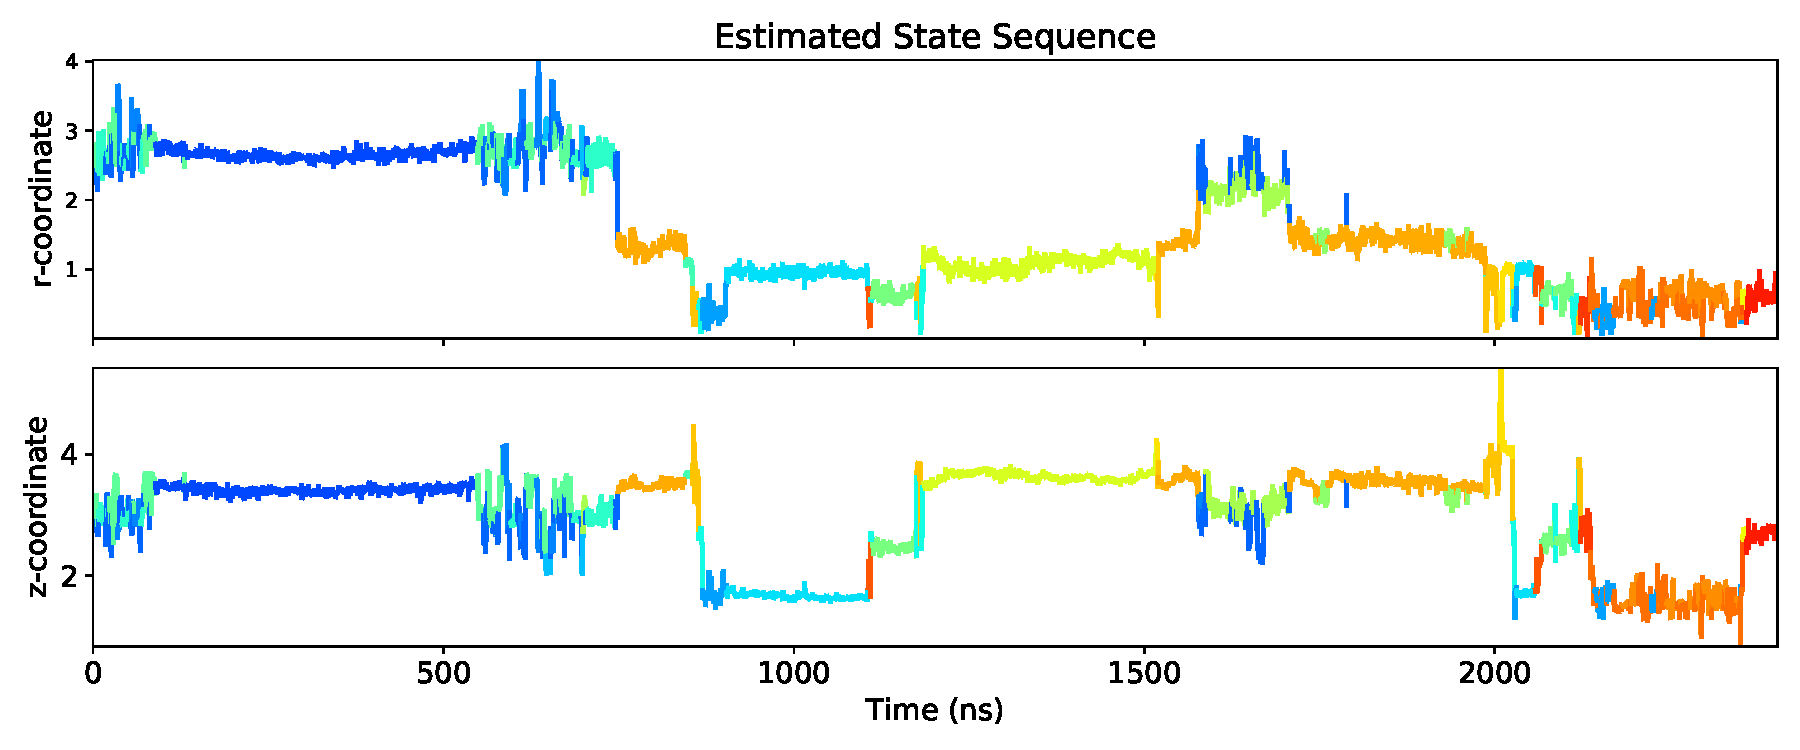
\includegraphics[width=\textwidth]{rz_unclustered_MET.pdf}
  \caption{The IHMM found 24 distinct VAR(1) states in this representative methanol trajectory.
  We performed the parameterization in 3D cartesian coordinates, but for this figure, we 
  converted to cylindrical coordinates, with $r$ the distance from the pore center, to 
  provide a clearer picture of solute motion.}\label{fig:rz_unclustered}
  \end{figure}
  
  \subsection{Reproducing MD Trajectories and MSDs with the IHMM}\label{section:unclustered_MSD_prediction}

  Before analyzing solute behavior characteristic to the states identified by the
  IHMM, it is important to verify whether the state dynamics are consistent with MD
  both qualitatively and quantitatively. Therefore, we generated stochastic 
  realizations based on the parameters of each trajectory as described in 
  Section~\ref{method:realizations}.
  
  As shown in Figure~\ref{fig:qualitative_unclustered}, realizations of our model 
  can produce trajectories that show qualitatively similar hopping and trapping 
  behavior to the MD trajectories to which they were fit. It is important that our
  model reproduces this behavior so that we can have confidence in its usefulness
  for quantitative predictions.
  
  % BJC4: This figure needs to be redone with new trajectory generation procedure
  \begin{figure}
  \centering
  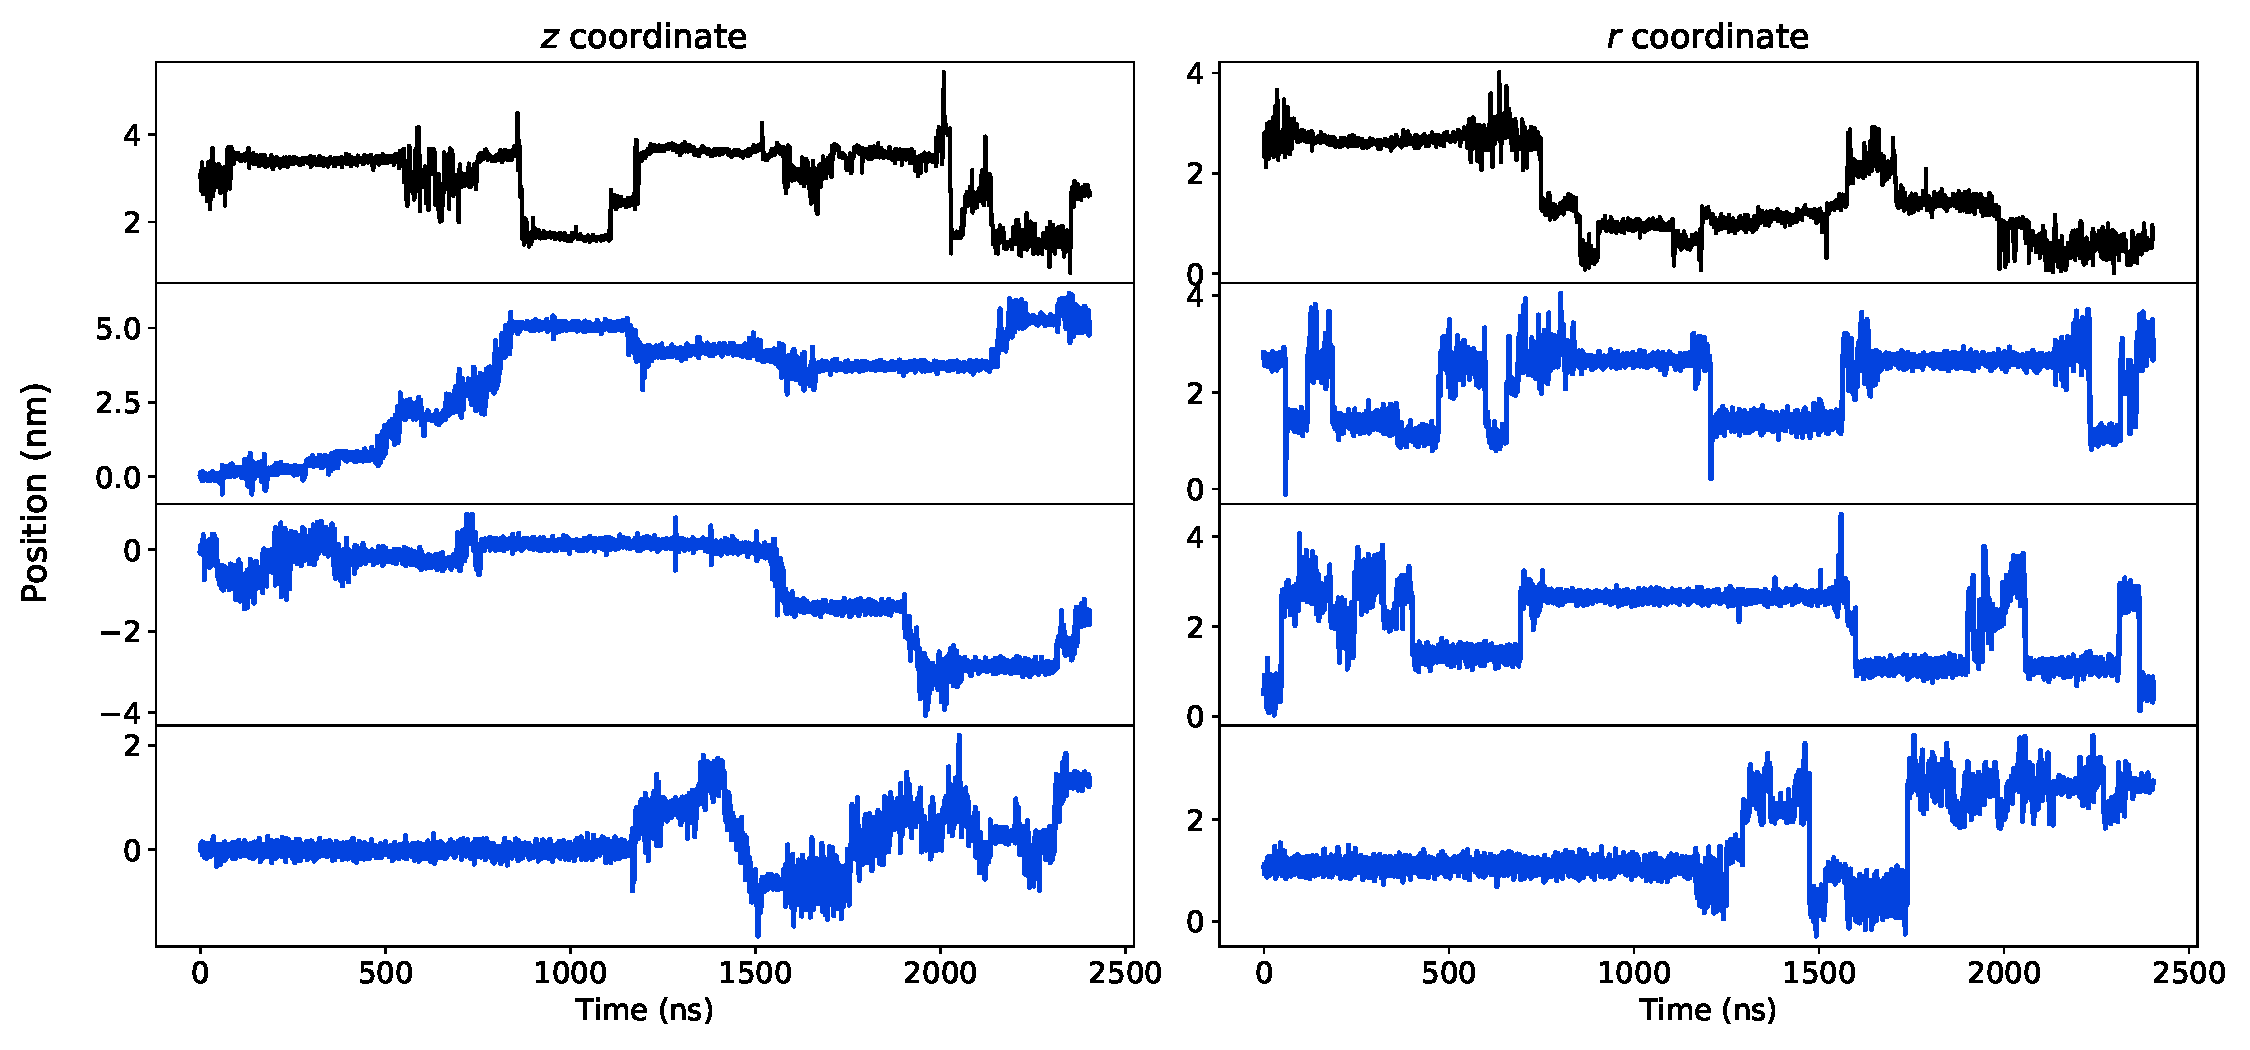
\includegraphics[width=\textwidth]{qualitative_unclustered_MET2.pdf}
  \caption{We can use realizations of the IHMM to generate trajectories which 
  bear qualitative resemblance to the MD trajectories. We used the parameters 
  of the IHMM, whose state segments are visualized in 
  Figure~\ref{fig:rz_unclustered}, in order to construct an ensemble of 
  characteristic trajectories. Solute trajectories generated with
  the IHMM (blue) show the same hopping and trapping behavior exhibited by 
  MD (black).
  }\label{fig:qualitative_unclustered}
  \end{figure}
  
  In Figure~\ref{fig:unclustered_msds}, we show that we can reproduce the 
  MD MSDs on long timescales within uncertainty using realizations of the 
  IHMM.
  \begin{itemize}
    \item We generated the MSD curves using Method 1 described in 
    Section~\ref{method:realizations} of the methods.
    \item Our ability to reproduce these curves gives use confidence
    in their long term predictions.
  \end{itemize}
  
  \begin{figure}
  \centering
  \begin{subfigure}{0.24\textwidth}
  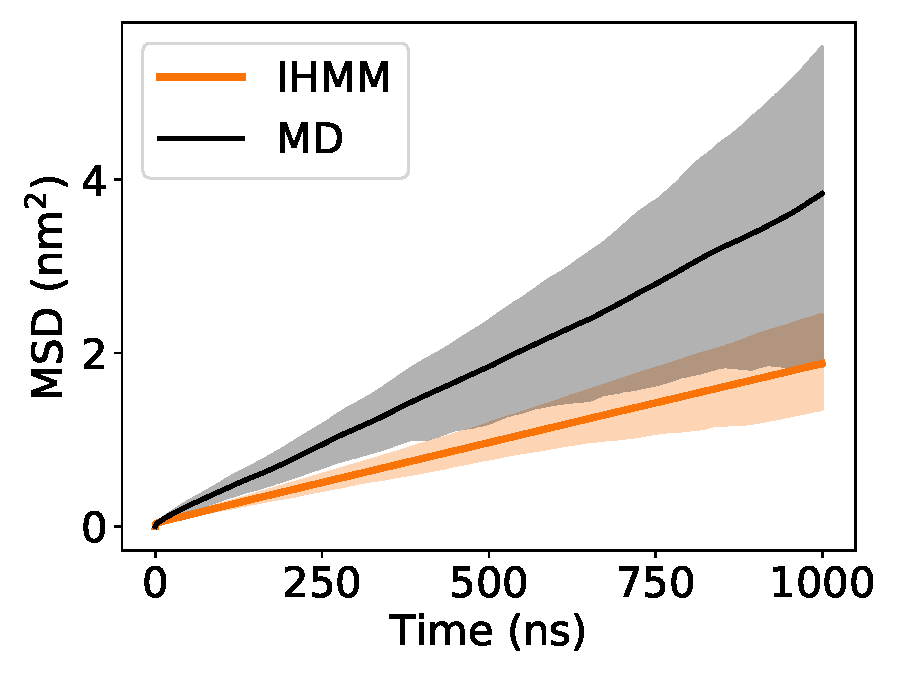
\includegraphics[width=\textwidth]{unclustered_msd_MET.pdf}
  \caption{methanol}\label{fig:unclustered_msd_MET}
  \end{subfigure}
  \begin{subfigure}{0.24\textwidth}
  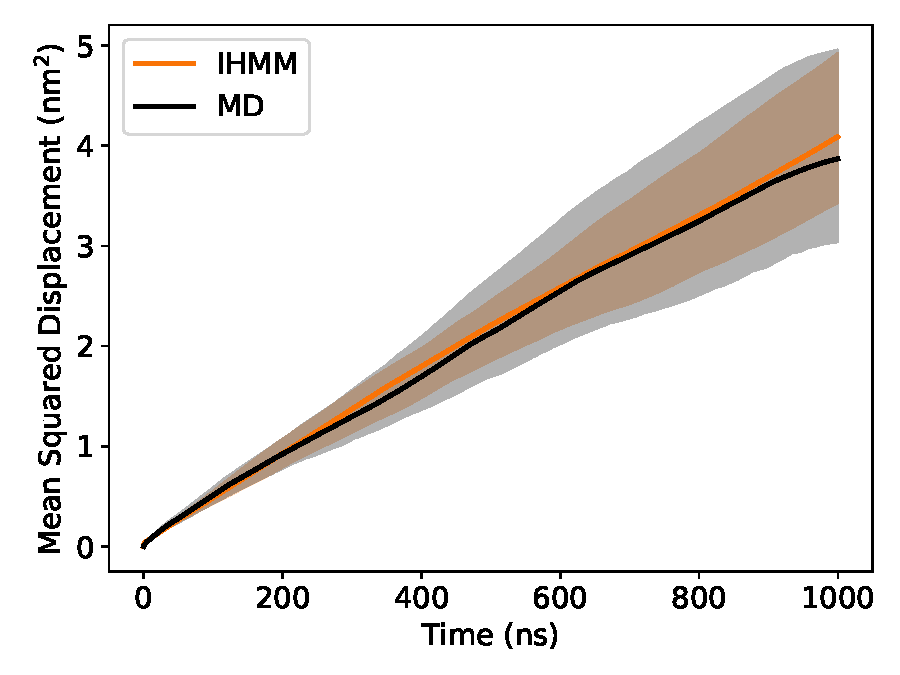
\includegraphics[width=\textwidth]{unclustered_msd_GCL.pdf}
  \caption{ethylene glycol}\label{fig:unclustered_msd_GCL}
  \end{subfigure}
  \begin{subfigure}{0.24\textwidth}
  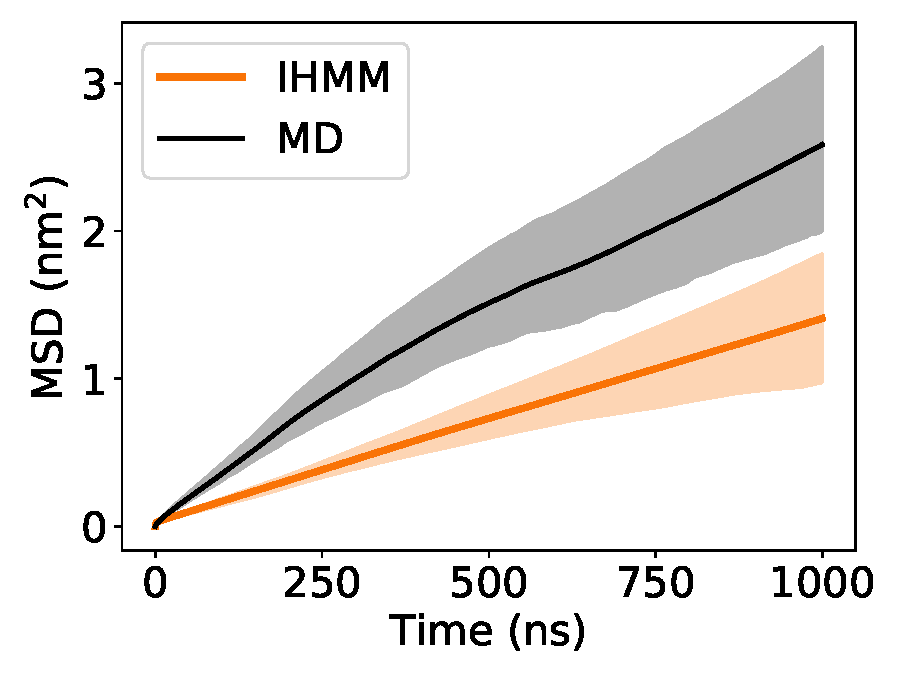
\includegraphics[width=\textwidth]{unclustered_msd_URE.pdf}
  \caption{urea}\label{fig:unclustered_msd_URE}
  \end{subfigure}
  \begin{subfigure}{0.24\textwidth}
  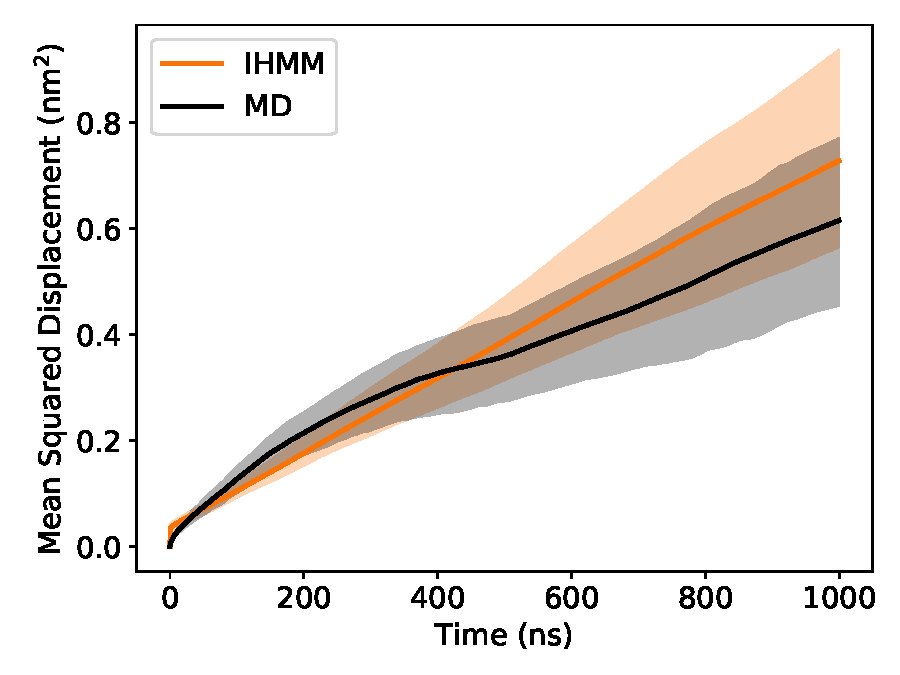
\includegraphics[width=\textwidth]{unclustered_msd_ACH.pdf}
  \caption{acetic acid}\label{fig:unclustered_msd_ACH}
  \end{subfigure}
  \caption{The MD MSDs (black) of methanol and urea are under-predicted by 
  the IHMM (orange), while the predictions match within uncertainty for ethylene
  glycol and acetic acid}\label{fig:unclustered_msds}
  \end{figure}
  
  \subsection{Using IHMM Parameters to Predict Selectivity}\label{section:macroscopic_properties}
  
  Since we can generate trajectories that share features similar to MD simulations, 
  it is now reasonable to project solute behavior onto much longer time scales.
  \begin{itemize}
    \item The IHMM MSD predictions quickly enter a linear regime, therefore we can 
    project long timescale MSDs based on the predicted diffusion constant as described
    in Section~\ref{method:selectivity}.
  \end{itemize}  
  
  %BJC4: figure here
  
  %BJC4: some kind of brief selectivity analysis here
  
  \subsection{Learning Mechanisms from the IHMM}\label{section:mechanisms}
  
  Solutes in this system show a wide range of behavior influenced by the 
  heterogeneity of the membrane's nanostructure as well as the interactions 
  between monomer and solute chemical functionality. Our application of the 
  IHMM can identify and distinguish these behaviors. The following approach 
  to analysis demonstrates how one can discover and explain the very complex
  behavior exhibited by solutes over long MD trajectories in terms of 
  solute-membrane interactions.
  
  \textit{State Clustering}: In order to reduce the state space to a more 
  manageable size, and to allow different solute trajectories to share 
  similar behavior, we clustered the states identified by the IHMM for each
  solute as described in Section~\ref{method:clustering}. In 
  Figure~\ref{fig:clustered_traj_MET}, we show the results of clustering on the 
  same methanol trajectory from Figure~\ref{fig:rz_unclustered}. Based on 
  the criteria described in Section~\ref{method:clustering},
  we chose to reducing the total state space for methanol from 287 to \nclusters. 
  
  Our goal is to derive the simplest model which adequately distinguishes
  different types of solute motion. By working to understand the parameters of 
  each cluster, we can uncover the associated transport mechanisms responsible
  for those parameters.
  
  \begin{figure}
  \centering
  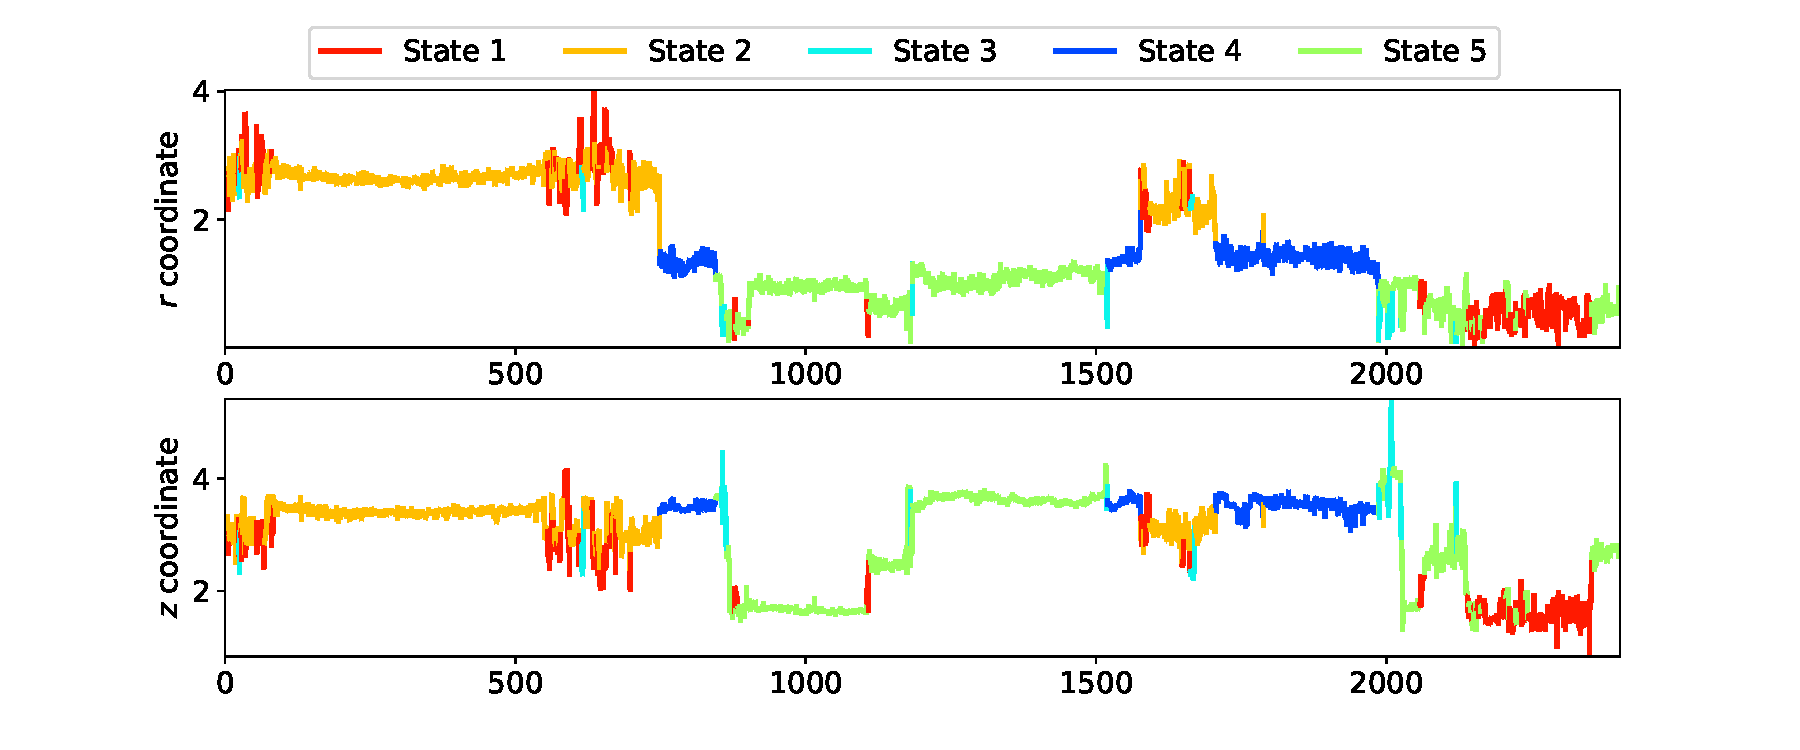
\includegraphics[width=\textwidth]{clustered_traj_MET_ward_10.pdf}
  \caption{We reduced the total state space from 287 to 10 total states 
  shared across all trajectories. For the trajectory in this figure, we reduced
  the total number of states from 24 (see Figure~\ref{fig:rz_unclustered}) to
  5.}\label{fig:clustered_traj_MET}
  \end{figure}
  
  \textit{Dynamics of clustered parameter sets}: The clustered parameter sets
  allow transitions between dynamics exhibited by the same solute from independent 
  trajectories. This allows us to create hybrid trajectories which draw on all
  solute behavior.
  
  Realizations based on the 10 clustered parameter sets do not show the same
  qualitative dynamics as the MD simulation trajectories. 
  \begin{itemize}  
    \item In Figure~\ref{fig:qualitative_clustered_MET}, we compare MD 
    trajectories to realizations of our model using the clustered parameter sets.
    \item They lack the diversity of behavior which we see in the MD simulation trajectories.
    \item They do not show the same range of trapping times and hop lengths.
    \item If we use a higher number of clusters, the qualitative match improves, but
    at the cost of a larger state space to interpret (see Figure~\ref{S-fig:qualitative_improvement}
    of the Supporting Information).
  \end{itemize}
  
  In addition to qualitative mismatches, realizations of the clustered IHMM 
  under-predict the unclustered MSD predictions and the MD MSD. 
  \begin{itemize}
    \item Much of a solute's MSD is likely a consequence of short-lived trapping states
    with high variances.
    \item When clustering, disjoint segments with similar enough parameters are
    re-parameterized together as part of the same state, lengthening the lifetimes 
    of very short-lived states and suppressing the fluctuations of high variance states.
    \item In Figure~\ref{fig:clustered_MSD}, it is evident that increasing the number
    of clusters increases the predicted MSD.
    \item Matching the unclustered MSDs would likely require many more clusters, at 
    which point the benefits of clustering are lost. 
    %BJC: I don't think the following discussion is necessary anymore.
%    \item In Figure~\ref{fig:dwell_distributions}, we compare the overall dwell time
%    distributions generated directly from MD simulations to that generated from 
%    realizations of the IHMM. 
%    \item We do this by measuring the time spent in each independent same-state segment.
%    \item Some of the probability density of short trapping times in the MD simulations 
%    gets shifted to medium length trapping times in realizations of the IHMM. 
%    \item In Figure~\ref{fig:dwell_distributions_modT} and~\ref{fig:msd_modT}, we show 
%    that by modifying the transition matrix to encourage transitions towards states with
%    shorter dwell times, we can more closely reproduce the dwell time distribution and 
%    MSD of MD. This is because most solute motion is a consequence of transitions between
%    trapped states.
  \end{itemize}
  
  \begin{figure}
  \centering
  \begin{subfigure}{0.63\textwidth}
  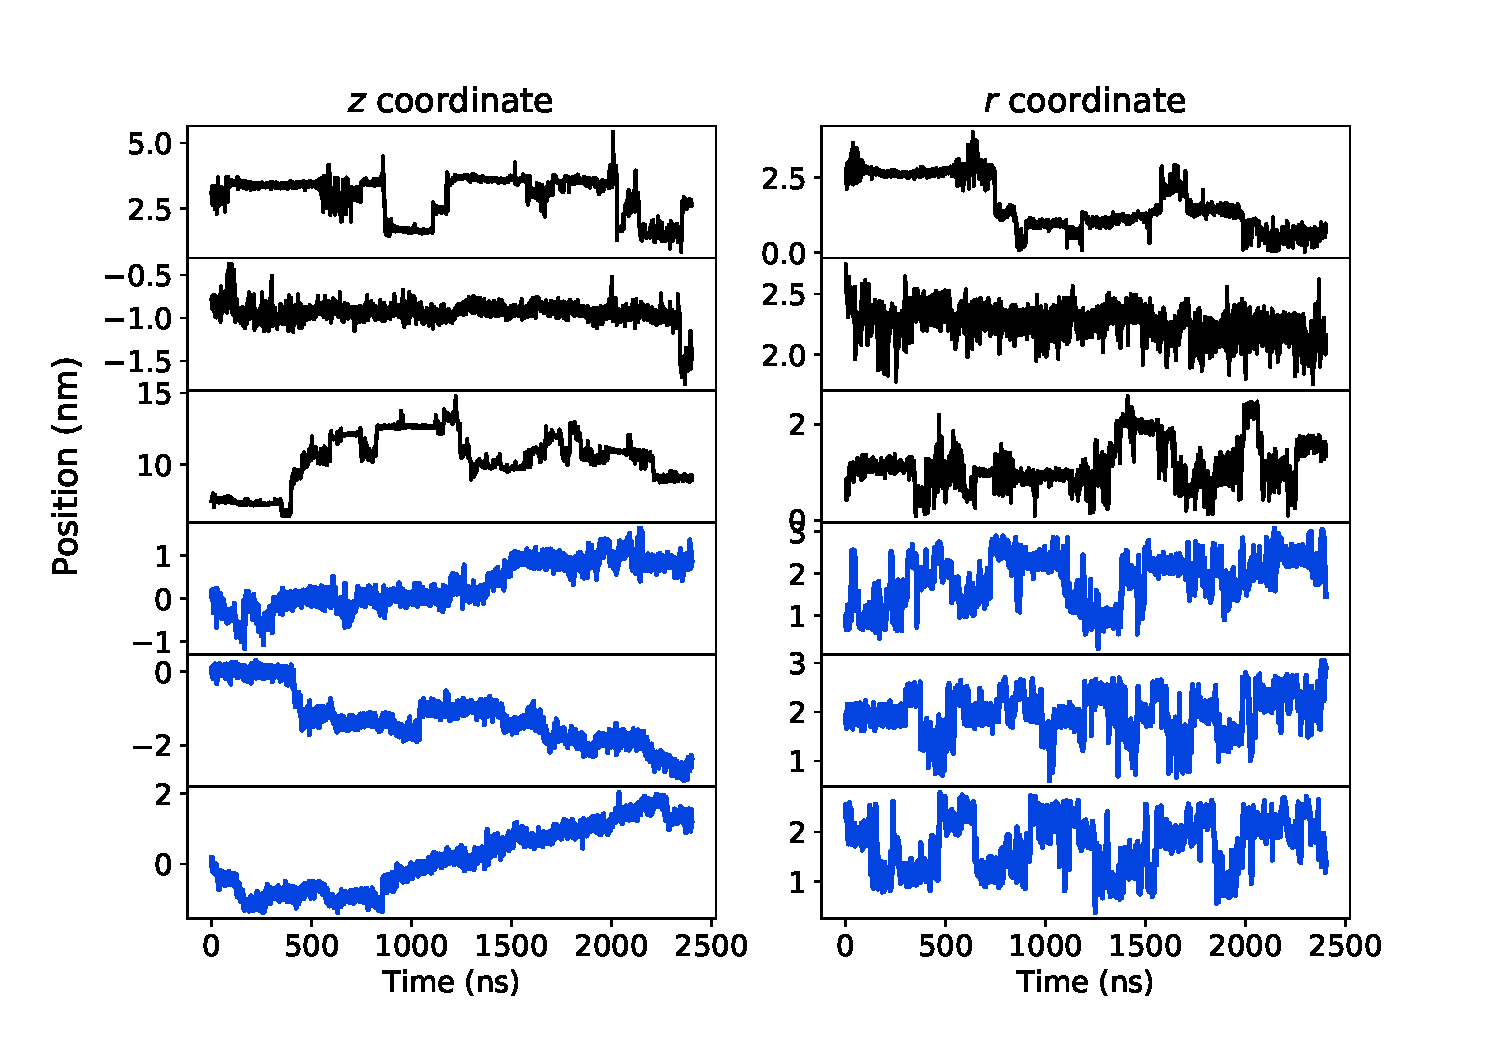
\includegraphics[width=\textwidth]{qualitative_clustered_MET_10.pdf}
  \caption{}\label{fig:qualitative_clustered_MET}
  \end{subfigure}
  \begin{subfigure}{0.35\textwidth}
  \vspace{2.25em}
  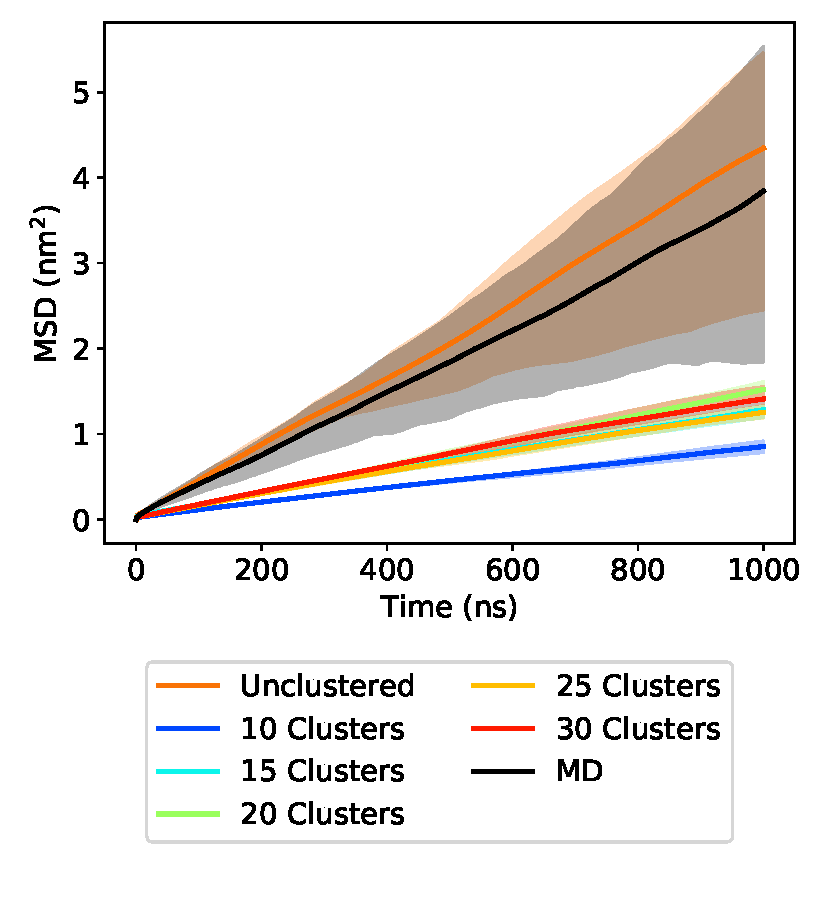
\includegraphics[width=\textwidth]{msd_nclusters.pdf}
  \caption{}\label{fig:clustered_MSD}
  \end{subfigure}
  \caption{(a) Stochastic trajectory realizations generated from our model (blue) based on
  the clustered methanol parameters do not qualit}\label{fig:clustered_dynamics}
  \end{figure}
    
%  \begin{figure}
%  \centering
%  % BJC4: combine (a) and (b). Add figure with MSD prediction
%  \begin{subfigure}{0.32\textwidth}
%  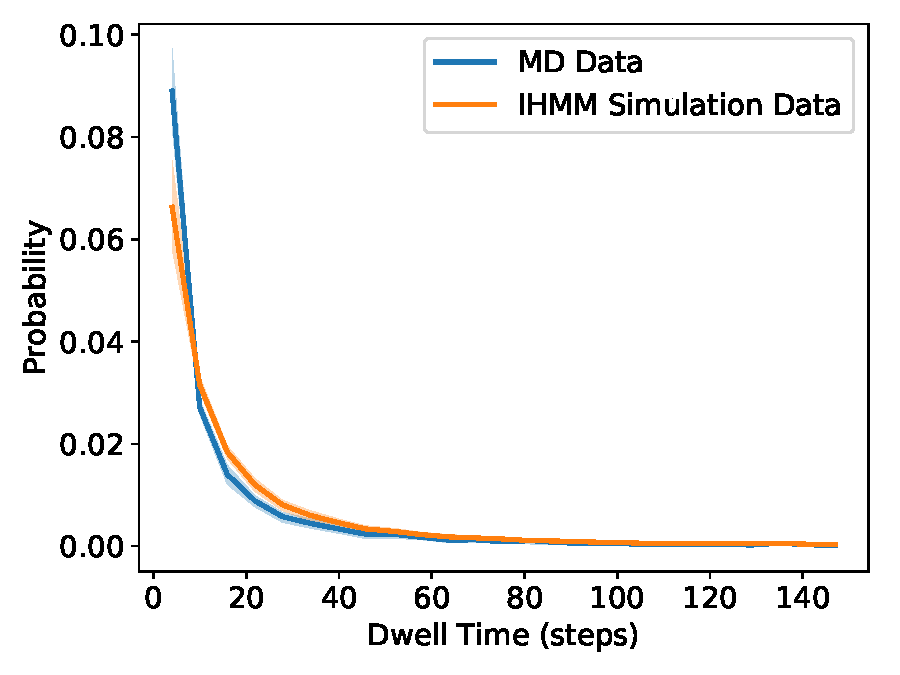
\includegraphics[width=\textwidth]{dwell_distributions.pdf}
%  \caption{}\label{fig:dwell_distributions}
%  \end{subfigure}
%  \begin{subfigure}{0.32\textwidth}
%  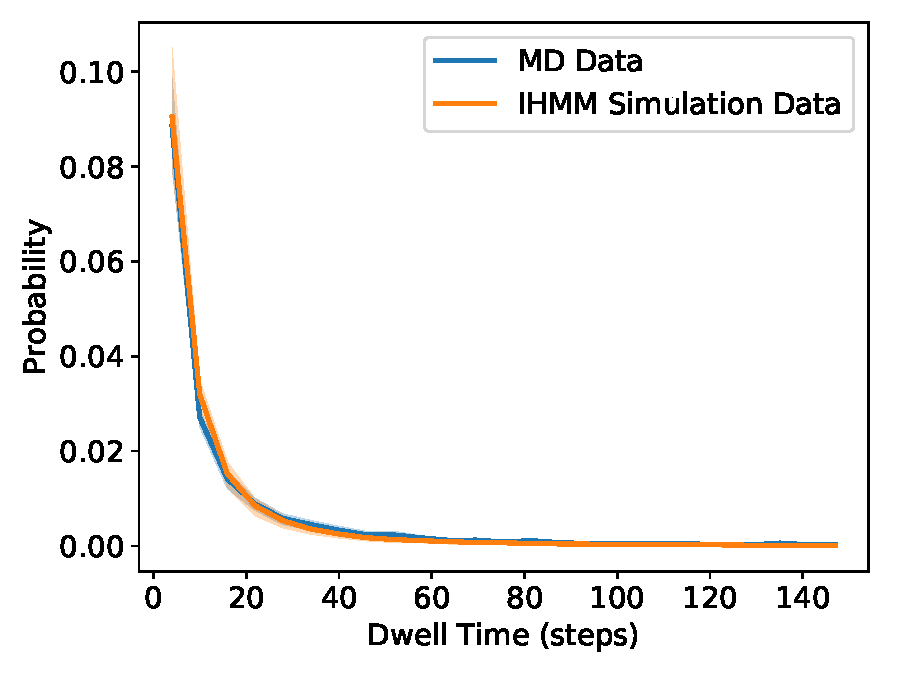
\includegraphics[width=\textwidth]{dwell_distributions_modT.pdf}
%  \caption{}\label{fig:dwell_distributions_modT}
%  \end{subfigure}
%  \begin{subfigure}{0.32\textwidth}
%  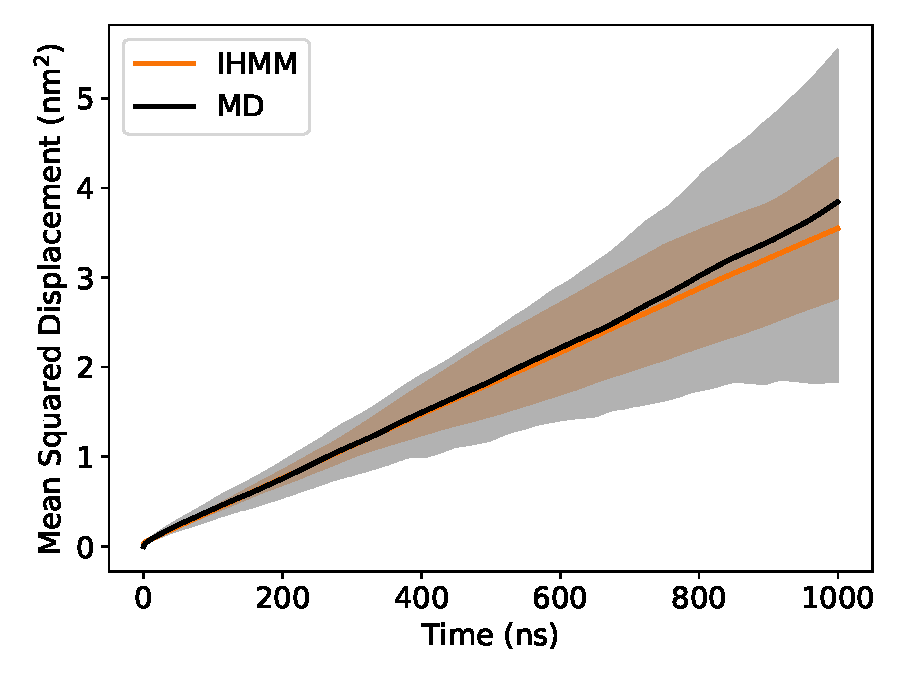
\includegraphics[width=\textwidth]{unclustered_msd_MET_modT.pdf}
%  \caption{}\label{fig:msd_modT}
%  \end{subfigure}
%  \caption{(a) The density of short dwell times compiled from realizations of
%  the IHMM fit to methanol trajectories is below that measured directly from 
%  the MD trajectories. If we modify the transition matrix in order to favor 
%  transitions towards states with short dwell times, we can more closely match
%  the (b) dwell time distributions and (c) MSDs.}\label{fig:slow_T}
%  \end{figure}
  
% BJC: probably a bad idea
%  It may still be possible to use these hybrid trajectories in order to predict
%  selectivity since they undershoot the MD MSD by a consistent number and 
%  the ratios will stay the same.
  
  % BJC2: the numbers and choices of states in this paragraph will change, but I think we
  % can still use this framework to study mechanisms.

%  \subsubsection*{Relating Clusters to Mechanisms}
%  
%  The parameters of each cluster can be related to dominant solute-membrane interactions.
%  \begin{itemize}
%    \item Based on our previous work, we know that hydrogen bonding, sodium ion 
%    association and radial location within the membrane pores will have a significant
%    influence on transport properties. 
%    \item Even without our previous work, it would still be easy to speculate that these 
%    interactions might occur and could therefore be used to help understand the 
%    states identified by the IHMM.
%    \item We have also incorporated membrane density as a physical metric because we 
%    know the membrane has an inhomogeneous structure.
%  \end{itemize}
  
%  \textit{Learning from individual trajectories}: In Figure~\ref{fig:mechanism_map}, 
%  we demonstrate the wide range of behavior exhibited by a representative 2D methanol
%  trajectory.
%%BJC2: reducing duplication
%%  The coordinates
%%  are colored according to the cluster with which methanol's dynamics are most consistent,
%%  which implies that this particular methanol trajectory exhibits eight distinct dynamical 
%%  behaviors (in order of their first appearance, they are colored dark yellow, red, light
%%  blue, light green, orange, blue, teal and lime green).
%  The solute time series are coupled with color coded bars which describe the solute's
%  local environment and physical interactions that it undergoes at each trajectory frame. 
%%  From the top, they describe 
%%  whether the solute is associated with sodium, whether the solute is hydrogen bonding
%%  with the monomer as well as to what part of the monomer it is hydrogen bonding, and 
%%  finally, the local number density surrounding the solute. 
%
%  %BJC2: the exact figure will change, but most of what I say shouldn't
%  \begin{figure}
%  \centering
%  \begin{subfigure}{0.75\textwidth}
%  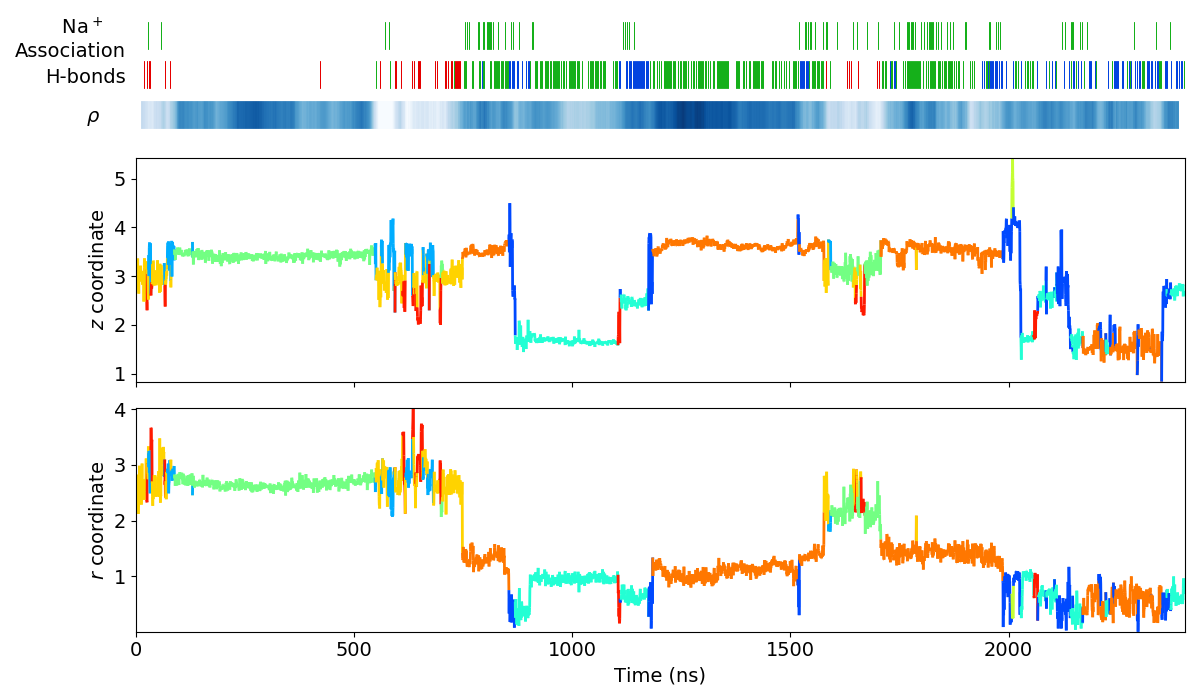
\includegraphics[width=\textwidth]{mechanism_map.png}
%  \caption{}
%  \end{subfigure}
%  \begin{subfigure}{0.24\textwidth}
%  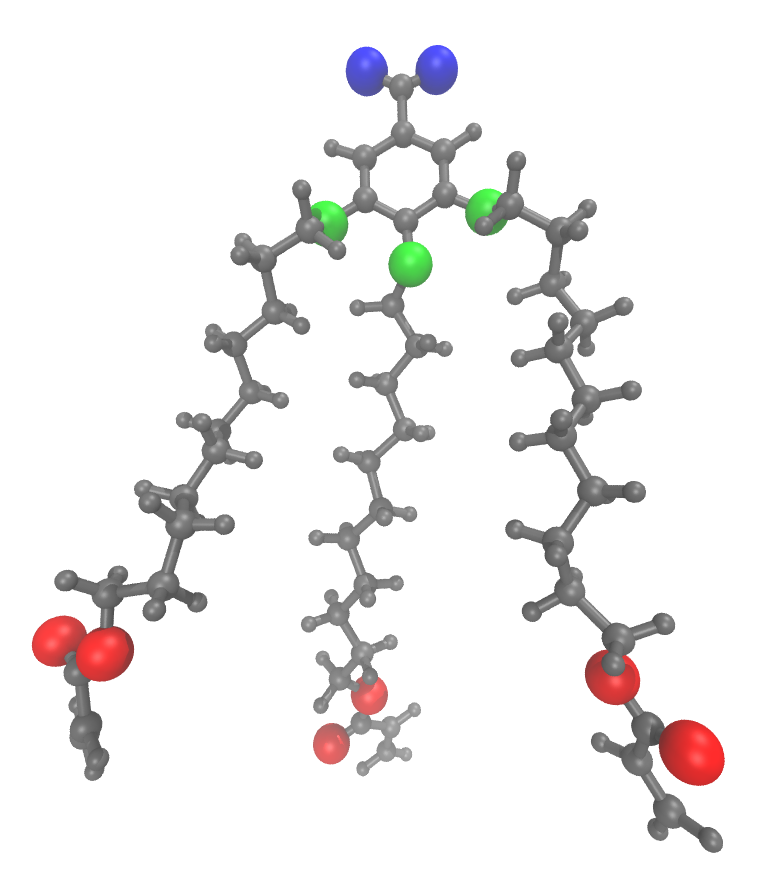
\includegraphics[width=\textwidth]{monomer_oxygens.png}
%  \caption{}
%  \end{subfigure}
%  %MRS: a lot of this caption test is duplicated from the main text. I would suggest reducing the duplication.
%  %BJC: you think better to have more detail in text or in caption?
%  %MRS2: at a certain point, it should be in the text.  In the caption, I would just state what the point of the plot is, 
%  % and define the colors/data/etc.  But full explanation would be better in the text. Captions should be scannable quickly,
%  % based on how people process papers, and this should be significantly shorter for readability. 
% \caption{(a) We can learn a significant amount of detail about solute motion by viewing 
%  solute trajectories color-coded according to their clustered dynamical behavior alongside
%  plots of the dominant molecular interactions and descriptions of the membrane's local 
%  environment. In the plot above, we show the radial and axial coordinates of a single
%  methanol molecule over the course of the equilibrated portion of its MD simulation.
%  Disjoint segments of the same color imply the solute behaves similarly at different 
%  points of the trajectory because their VAR parameters place them in the same cluster. 
%  There are eight distinct dynamical modes exhibited by this trajectory. In order
%  of their first appearance, they are colored dark yellow, red, light blue, light green,
%  orange, blue, teal and lime green. On the top of the plot are bars which represent different
%  physical interactions and the membrane's local environment as a function of time. The top 
%  bar is colored green at time points where solutes are associated with sodium. Methanol 
%  associates with sodium ions relatively infrequently. The next bar down is colored when hydrogen
%  bonds exist. The colors match the enlarged oxygen atoms highlighted in (b). Blue slivers
%  correspond to hydrogen bonds donated to the monomer's carboxylate head group. Green slivers
%  correspond to  hydrogen bonds donated to the ether linkages between the head groups
%  and tails. Red slivers correspond to hydrogen bonds donated to the oxygens on the ends
%  of the monomer tails. Methanol exhibits significant hydrogen bonding with all parts of
%  the monomer. Which part of the monomer methanol hydrogen bonds to is heavily correlated
%  to the solute's $r$ coordinate. Finally, the bar with the blue gradient represents the local 
%  membrane density based on the solute's ($r$, $z$) coordinate. Darker shades of blue
%  correspond to higher membrane densities. The density appears to be higher when methanol
%  motion is restricted (e.g. from 75 to 550 ns). It is relatively low in areas where methanol's
%  position fluctuates significantly (e.g. from 550 to 700 ns). 
%  }\label{fig:mechanism_map}
%  \end{figure}
%
%  One can gain useful chemical intuition just by studying plots like 
%  Figure~\ref{fig:mechanism_map}. It is clear that, for methanol, association 
%  with sodium is a much rarer interaction than hydrogen bonding with the 
%  LLC monomers. Methanol hydrogen bonds to all regions of the monomers dependent
%  on its radial position. Its fluctuations tend to be smallest when hydrogen bonded
%  or in areas of high local number density. For example, from approximately 75 to 
%  525 ns, methanol appears to be trapped in a high density region of the tails.
%  In the time that follows, it enters a region of relatively low density where 
%  fluctuations are quite large. During this time period, there is intermittent, 
%  short-lived hydrogen bonding with the oxygen atoms at the tail ends, as suggested
%  by the frequent state changes during that time period and red slivers in the bar
%  above. Significant hops in the $z$ direction appear to be described by the dark blue
%  state. After entering the dark blue state ca. 850 ns, methanol appears to jump
%  significantly in the $z$ direction from a hydrogen bonded state with the ether 
%  linkages to a hydrogen bonded state with a head group in a monomer below it.

  
  \textit{The dynamics of frequently occurring states}: We may learn the most by 
  studying the dynamical modes common to the majority of the solute trajectories.
  \begin{itemize}
  	\item Of the 10 state clusters, only 5 appear in a significant number of 
  	solute trajectories (Figure~\ref{fig:prevalence}).
  	\item Although a majority of the solutes visit these 5 states the
  	amount of time spent in each varies widely. 
  \end{itemize} 
  
  \begin{figure}
  \centering
  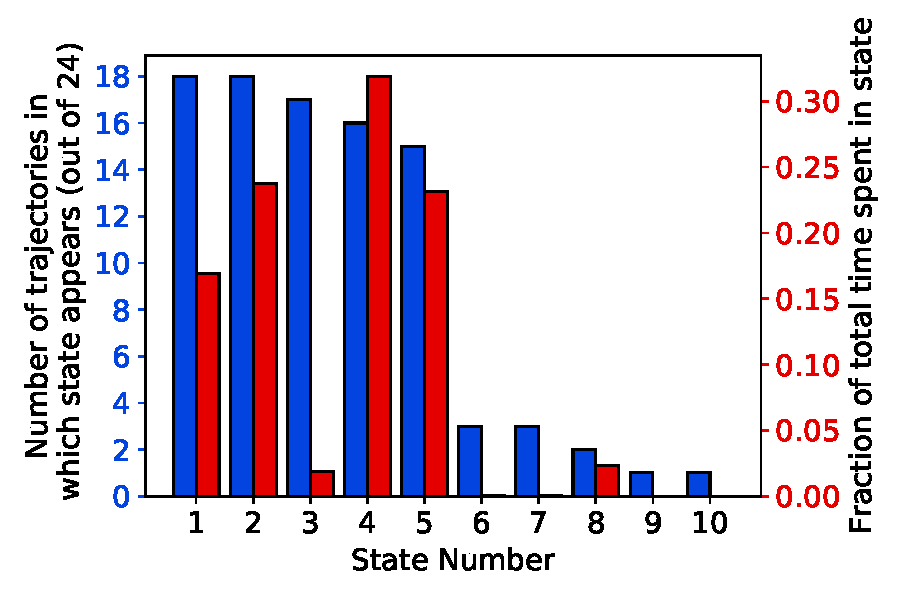
\includegraphics[width=0.5\textwidth]{prevalence.pdf}
  \caption{5 out of the 10 clustered states are visited by 15 or more of the solute
  trajecotries. The solutes spend varying amounts of time in each of these states.
  }
  \label{fig:prevalence}
  \end{figure}
  
  We can begin to hypothesize mechanisms by studying the behaviors defined by the 
  state parameters.
  \begin{itemize}
  	\item In Figure~\ref{fig:common_states_lines}, we plot representative 
  	dynamics of each of the five most visited states.
  	\item The states exhibit a range of autoregressive and trapping behavior
  	throughout the membrane pores.
%  	\item There is good representation by states across a range of radial distances
%  	from the pore centers. 
  \end{itemize}
  
  Since the radial means are weighted averages of the states used to parameterize
  each cluster, for interpretive purposes, it is important to recognize that the means
  only provide clues towards the general location of the solute. 
  \begin{itemize}
  	\item For example, the radial mean of state 3 is 1.4 nm from the pore center. 
  	\item However, inspection of Figure~\ref{fig:clustered_traj_MET} suggests that this 
  	type of behavior actually occurs radially throughout the pore.
  	\item There are instances of state 3 less than 1 nm from the pore center and more 
  	than 2 nm from the pore center. 
  	\item In this case, the radial mean only suggests that this type of behavior 
  	happens in both regions somewhat equally.
  \end{itemize}
  
  Solutes exhibit a range of autoregressive behavior as shown by the representative 
  solute trajectories in Figure~\ref{fig:common_states_lines} and the scatter
  plot in Figure~\ref{fig:A_sigma_scatter}.
  \begin{itemize}
  	\item In most cases, the eigenvalues of $A$ and $\Sigma$ appear nearly paired
  	in their radial and axial dimensions, which implies nearly symmetric behavior 
  	with off-diagonals both matrices near zero.
  	\item The most notable exception is state 3, which has a much higher radial 
  	eigenvalue of the covariance matrix.
  	\item Both eigenvalues are actually of state 3's covariance are actually quite
  	large. This implies relatively large fluctuations in the $z$ direction and even
  	bigger fluctuations in the $r$ direction.
  	\item All states have slightly lower covariance in the axial direction. It's
  	likely easier for solutes to move laterally rather than to move up through the
  	alkane chains.
  	\item States 3 and 4 show a strong previous-hop dependence (high $A$) while
  	the rest of the states have a somewhat weaker dependence.
  \end{itemize}

  Solutes are trapped for various lengths of time.
  \begin{itemize}
    \item On average, state 4 has the longest dwell times and state 3 has
    the shortest dwell times while the rest have intermediate dwell times.
    \item This is partially confirmed via inspection of Figure~\ref{fig:clustered_traj_MET},
    however. 
    \item Once again, since we clustered, it is important to avoid distraction
    by the exact dwell time values, and to focus on their relative magnitudes
  \end{itemize}
  
  % BJC4: Not sure if this is useful. Maybe can replace above three paragraphs 
  % with this. Helps us look for mechanisms.
  By studying the parameters, it is now easier to describe the state behavior.
  \begin{enumerate}[label={State \theenumi :}, leftmargin=3.5\parindent]
     \item This state has intermediate dwell times with high past-hop dependence.
     The radial mean and evidence from Figure~\ref{fig:clustered_traj_MET} suggests
     that this state is common in the tail and pore region.
     \item This state seems to occur exclusively in the tail region based on its radial
     mean. Its fluctuations are small and there is little past hop dependence
     \item This is likely a hopping state that strongly contribute to the solute's MSD. 
     It is short lived and takes very large hops. This type of behavior is exhibited 
     near and far from the pore center as discussed earlier.
     \item This is a trapping state with a strong dependence on its previous fluctuation.
     Evidence from Figure~\ref{fig:clustered_traj_MET} and a radial mean of 1.8 suggest
     that it tends to occur at intermediate distances from the pore center.
     \item This is an intermediate-length trapping state that occurs close to the pore
     center. It's fluctuations are tight and relatively independent of its previous 
     fluctuation.
  \end{enumerate}
  
  \begin{figure}
  \centering
  \begin{subfigure}{0.58\textwidth}
  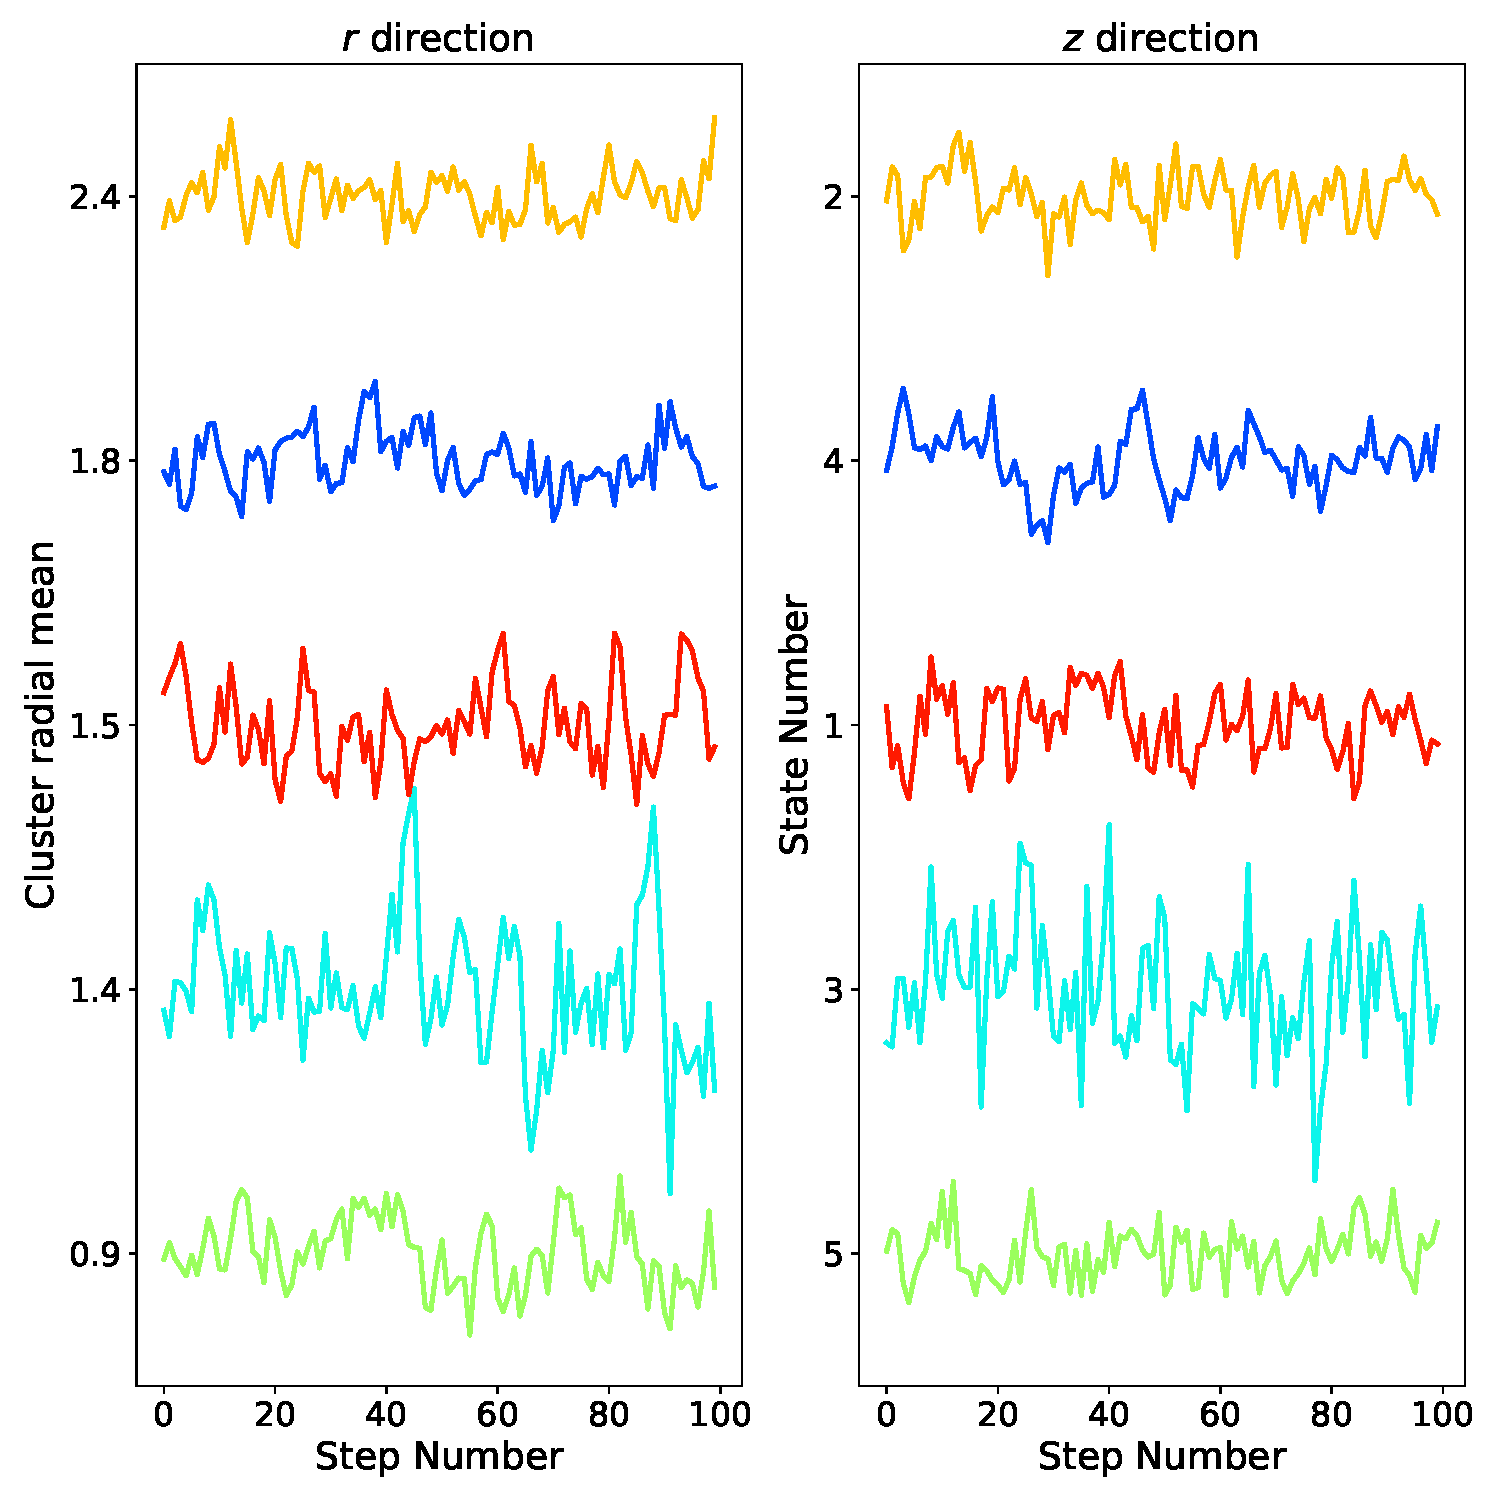
\includegraphics[width=\textwidth]{common_states.pdf}
  \caption{}\label{fig:common_states_lines}
  \end{subfigure}
  \begin{subfigure}{0.41\textwidth}
  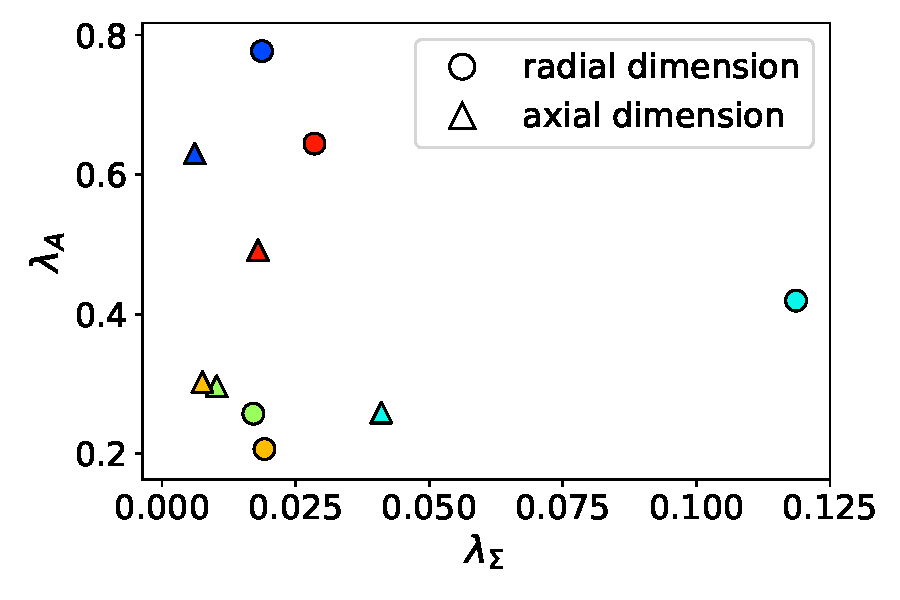
\includegraphics[width=\textwidth]{A_sigma_scatter.pdf}
  \caption{}\label{fig:A_sigma_scatter}
  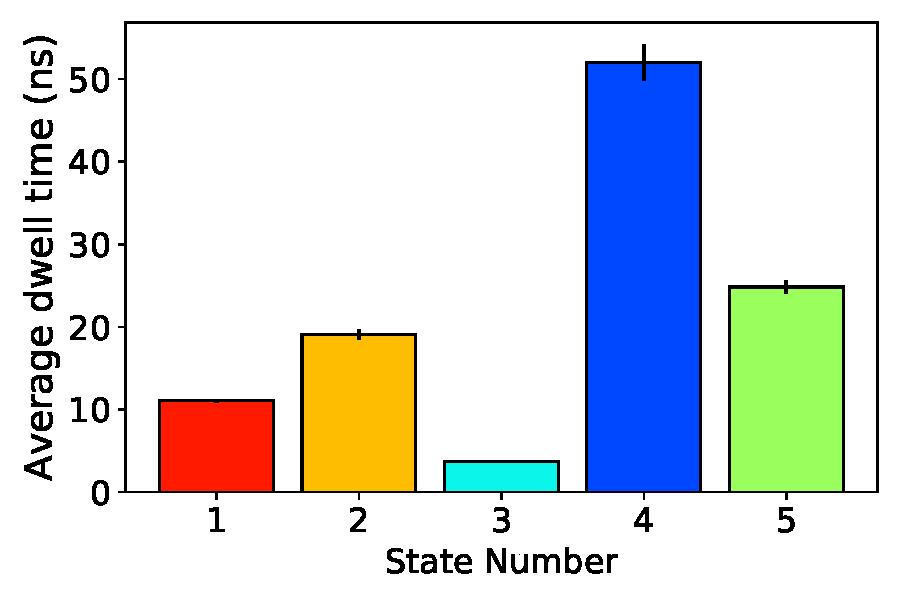
\includegraphics[width=\textwidth]{dwell_times.pdf}
  \caption{}\label{fig:dwell_times}
  \end{subfigure}
  \caption{The 5 most visited states by methanol show a range of dynamical behavior. In 
  (a), we show representative dynamics of these states. All time series have a mean of zero and are
  shifted to put the mean in line with the $y$-axis labels for the purpose of visualizing them.
  The $y$-axis labels of the $r$ coordinate plot specify the radial mean of each clustered 
  state. All of the states pictured appear in the trajectory shown in 
  Figure~\ref{fig:clustered_traj_MET} and are colored to match.
  (b) We can begin to understand the solute behaviors demonstrated in (a) by understanding their VAR 
  parameters. Higher values of $\lambda_{\Sigma}$ generally are indicative of large fluctuations
  and higher values of $\lambda_A$ indicate strong previous-hop dependence of the fluctuations.
  (c) Using Equation~\ref{eqn:dwell_times}, we estimated the expected time spent within each 
  of the states.
  }\label{fig:common_states_MET}
  \end{figure}
  
  % BJC2: Again, this will change, but will follow the same general flow
%  We can begin to dissect the dynamics of each state by studying their parameters.
%  States 1, 3 and 5 have radial means near 1 nm or less (see y axis of $r$ direction 
%  plot in Figure~\ref{fig:common_states_MET_lines}), which suggest that they occur
%  close to the pore centers. States 2, 4, 6 and 7 occur well within the tail region
%  of the membrane. States 1 and 2 have higher covariances in both the axial and radial
%  directions compared to all other states. Covariance in each dimension appears to have
%  a strong correlation. States 3 and 5 (in the pore region) as well as states 4, 6 and
%  7 (in the tail region) are primarily distinguished based on their autoregressive 
%  coefficients, A. Higher values of A generally lead to more wandering about the state
%  mean. One could argue that the parameters of states 3--7 are actually very close which
%  suggests that solutes might behave alike in morphologically distinct regions of the 
%  membrane.
%
%  Despite some similarity in their VAR parameters, the length of time spent in states 
%  3--7 appears to be dependent on the solute's radial location. Based on the 
%  self-transition probabilities, we estimated the average time spent by each solute in
%  each state (Figure~\ref{fig:dwell_times_MET}). States 3, 5 and 7 have long dwell times
%  relative to the rest because they have high self-transition probabilities. Somewhat 
%  surprisingly, both states 3 and 5 correspond to solutes located close to a pore center,
%  where one might expect solute motion to be less restricted. Although solutes in states
%  4 and 6 are in the viscous tail region, their dwell times are only intermediate. This
%  could be due to inhomogeneity in the tail region which causes transitions between many
%  different trapped states but with little net effect on solute MSD. However, there are
%  instances of states within the tail region with dwell times that exceed 100--200 ns,
%  as shown by our inclusion of state 7. There are no other states with dwell times longer
%  than state 5 in the pore region.
%  
%  States 1 and 2 exhibit the shortest dwell times of the states studied. This is 
%  consistent with the trajectory in Figure~\ref{fig:mechanism_map}. State 2 is the 
%  shortest lived state, appearing to bridge other tail region states. State 1 
%  appears to represent a significant hopping state. It has a high covariance and
%  occurs near the pore center, where there is less obstruction to solute motion.
%  It's dwell time of ca.~8 ns, suggests that solutes stay in this highly mobile 
%  state for long enough for their positions to displace significantly.
  
  \textit{Relating Parameters to Solute-Membrane Interactions}: Most of what we 
  have learned thus far has been based on the parameters of our model with some 
  qualitative validation using a single methanol trajectory. While 
  we may be able to further corroborate our arguments by analyzing more
  individual trajectories, it is more useful to correlate the state behavior with
  solute-membrane interactions.

  %BJC2: A lot of the following will probably be reworked with different clustering scheme
%  \textit{Hydrogen Bonding Patterns}: 
  The types of hydrogen bonding undergone by solutes is dependent on radial
  location (see Figure~\ref{fig:hbond_pichart}). States with radial means near 1 nm
  or less (states 1, 3 and 5) typically hydrogen bond with the monomer carboxylate
  groups and ether linkages. States with radial means greater than 1 nm (states 2,
  4, 6 and 7) tend to hydrogen bond with the monomer tails. Our previous work has
  shown that there is a gradual transition from the hydrophilic to hydrophobic region in
  these membranes, meaning the monomer location is not tightly bound in $r$. 
  %MRS: above logic is not clear?
  Therefore, there are instances of hydrogen bond interactions that one might consider 
  uncharacteristic based on the state's radial mean.
  %MRS: what is implication of ``uncharacteristicness''? 

  States which exhibit longer dwell times have longer hydrogen bond lifetimes (see
  Figure~\ref{fig:hbond_pichart}). States 3--7 have significantly longer hydrogen 
  bond lifetimes than states 1 and 2. It makes physical and mathematical sense that
  states 1 and 2 should not stay trapped by hydrogen bonding for long periods because
  they typically take large hops as communicated by their large covariances.
  In the tail states, hydrogen bond lifetimes appear to increase with their dwell 
  times. However, in the pores, the same linear relationship does not hold.
  For example, state 5 has the lowest hydrogen bond lifetime of states 3--7
  despite having the second longest dwell times. 
  
  The local density experienced by solutes may have an impact on the length of solute 
  entrapment. On average, solutes in state 5 are surrounded by a relatively high density
  of particles. Based on its radial location and preference towards hydrogen bonding
  with the ether linkages (see Figure~\ref{fig:hbond_pi_charts}), it is reasonable to
  assume that while in state 5, methanol spends most of its time just outside the 
  pore region, sandwiched between the monomer head groups. Although state 5 hydrogen
  bonds break more frequently than one might expect for a state with long dwell times,
  it is possible that the solute's dense surroundings prevent it from wandering off 
  before the hydrogen bonding interaction can be recovered. This may explain the 
  behavior of the methanol in state 5 of the trajectory in Figure~\ref{fig:mechanism_map}
  where the solute's center of mass appears to move more freely about its mean than 
  other trapped states. The data suggests that methanol molecules in state 3 lie closer
  to the pore center than state 5 because they tend to hydrogen bond most frequently 
  with the carboxylate groups. Methanol molecules which experience state 3 are subject 
  to a lower density local environment and rely more heavily on hydrogen bonding interactions, 
  evidenced by their longer lifetimes, to stay trapped.
  
  States describing behavior in the tail region show a direct relationship between 
  hydrogen bond lifetimes and local density. Methanol molecules which experience state 2 
  spend their time in a low density region of the tails where they can easily break free
  of hydrogen bonds. Conversely, methanol molecules trapped in state 7 are in the densest 
  region of all states studied. It is likely difficult for methanol to escape these high 
  density regions and its position is further stabilized via hydrogen bonding.
  
  %BJC4: I didn't put sodium ion association in this figure because it's infrequent. 
  %BJC4: If I compare to acetic acid or urea, I could add it back. I was thinking of splitting
  % the pi chart in half with slices corresponding to hbonds on one side and association on the other
  \begin{figure}
  \centering
  \begin{subfigure}{0.54\textwidth}
  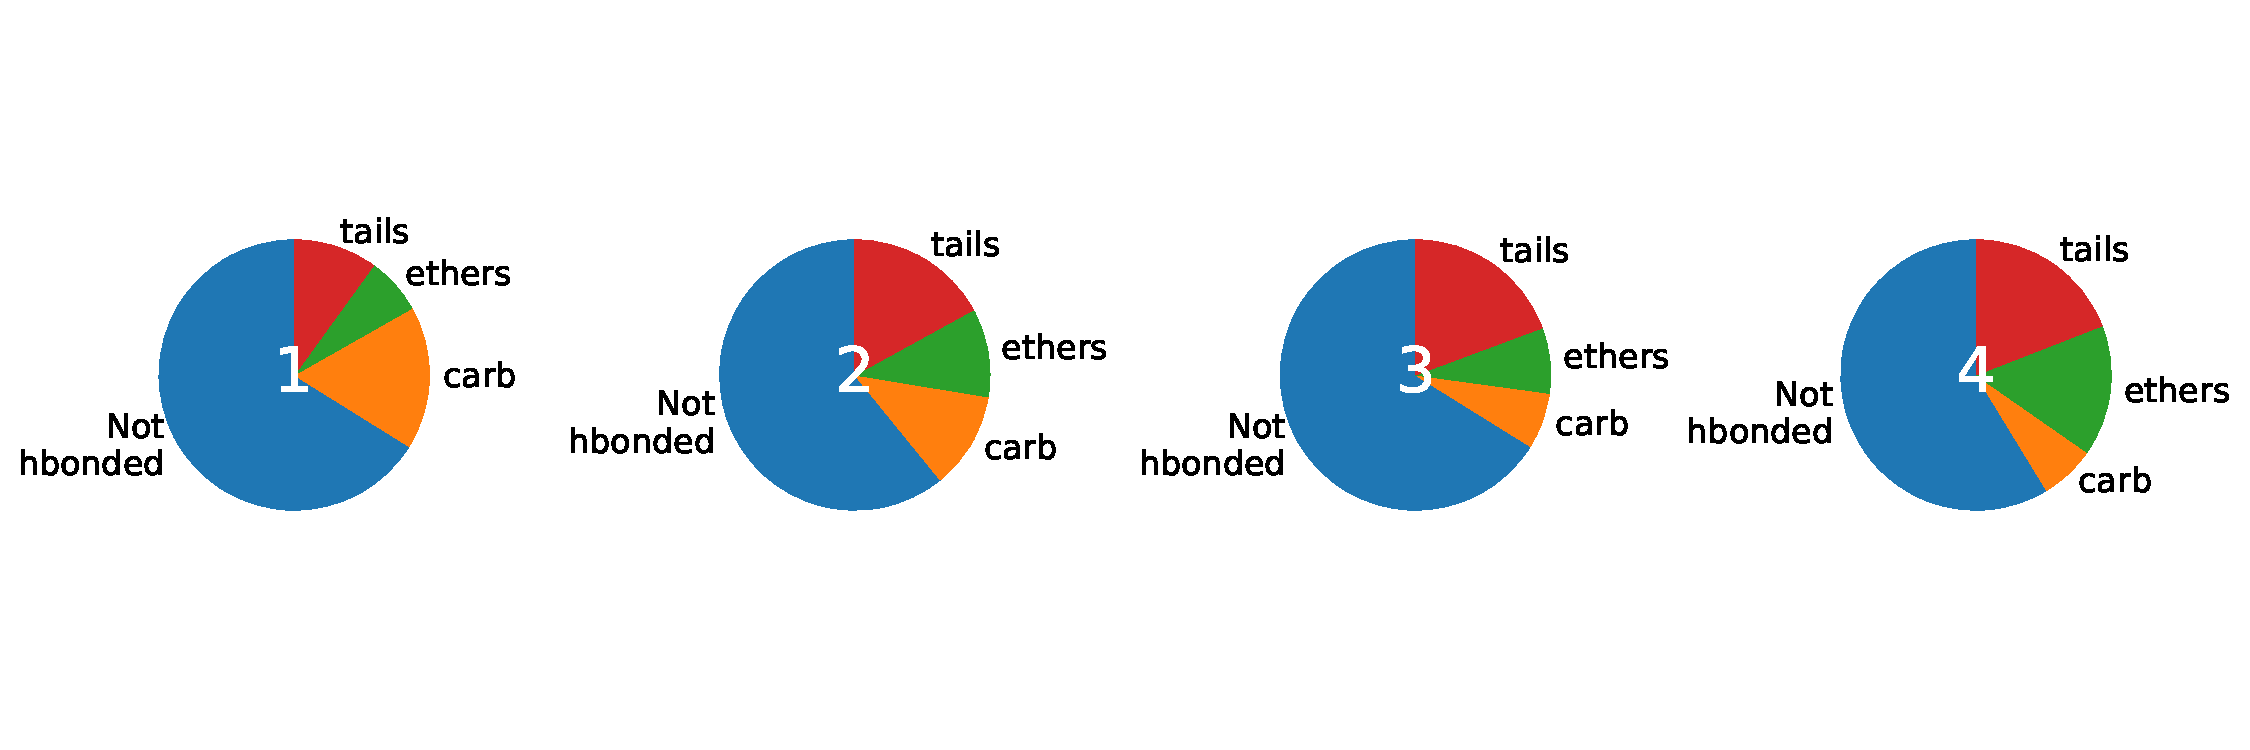
\includegraphics[width=\textwidth]{hbond_pi_charts.pdf}
  \caption{}\label{fig:hbond_pi_charts}
  \end{subfigure}
  \begin{subfigure}{0.45\textwidth}
  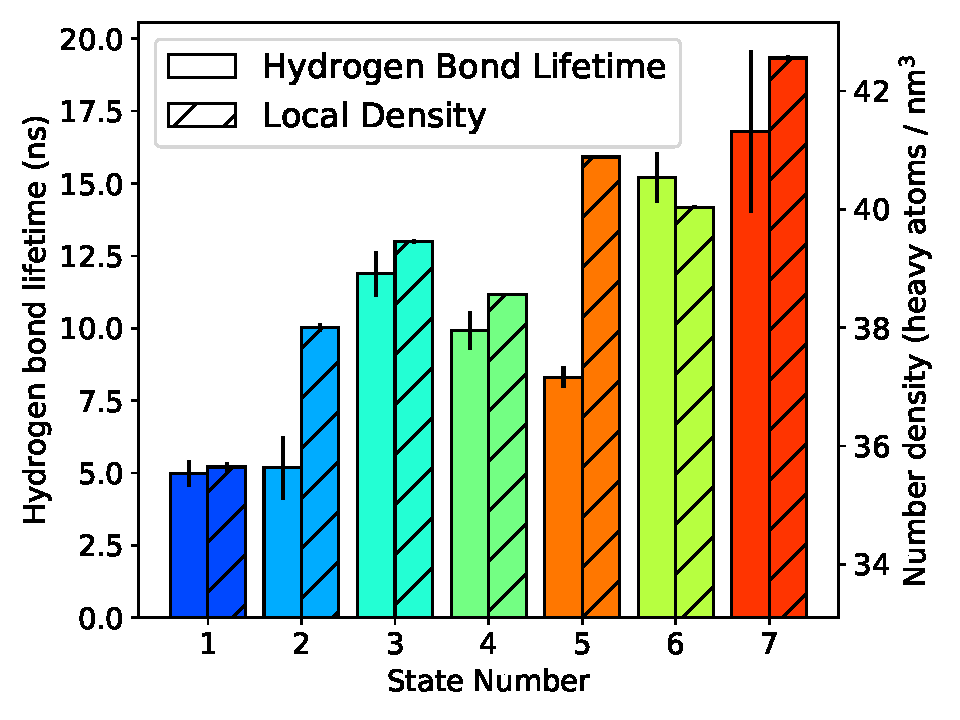
\includegraphics[width=\textwidth]{hbond_lifetimes_density_MET.pdf}
  \caption{}\label{fig:hbond_lifetimes_density_MET}
  \end{subfigure}
  %MRS: legend doesn't show stripes.
  \caption{(a) Methanol hydrogen bonds in different segments of the LLC monomer
  dependent on the state. States with mean radial locations in the pore region tend to
  hydrogen bond with the head groups and ether linkages. States with mean radial
  locations in the tails tend to hydrogen bond with the tail oxygen atoms.
  (b) Hydrogen bond lifetimes and the local density experienced by methanol
  molecules can help us to understand dynamical states in terms of membrane 
  interactions. The bars are colored according to match the states in Figures~\ref{fig:mechanism_map}
  and~\ref{fig:common_states_MET}. States 1 and 2, which have large covariances, also have short
  hydrogen bond lifetimes and exist in relatively low density regions. The
  hydrogen bond lifetimes of methanol in states with radial means in the tail
  region tend to increase with local density and mean dwell times. 
  %MRS7: not clear from graphic which ones are in the pore.
  %MRS7: is there any legend for the color for b? If same as above figure, indicate. Don't REALLY need color since they bars are already labeled, so it's 2 sources of duplicate information.
  %BJC7: The state numbers are all you need to compare to the previous figure BUT the color make it easier 
  %plot of the methanol trajectory where states aren't labeled.
  %MRS7: cross-hatching doesn't appear in the legend? Not sure which is which (I assume hatched is number density because closer to that axis).
  %BJC7: Is it because the hatches aren't dense enough? I see them in the legend
  This monotonic
  relationship does not exist for states in the pore region. The high 
  local density experienced by state 5 methanol molecules may explain why 
  hydrogen bond lifetimes are short but dwell times are high. State 5 methanol's
  preference towards hydrogen bonds with ether linkages suggests that the solute
  sits between LLC monomer head group which prevent it from wandering to far
  before recovering its previous hydrogen bond.
  }\label{fig:hbond_pichart}
  \end{figure}
  
  \subsubsection*{Comparison of Solute Behavior}
  %BJC2: Again, most of this section will get a facelift, but will try to follow same flow 
  We applied similar analysis to the other three solutes in this study: urea, acetic acid
  and ethylene glycol. Not only can we use the model to study the dynamics of each 
  solute individually, but we can compare their behavior in order to improve our
  understanding of more subtle mechanistic details.
  
  The size and chemical functionality of the solutes dictates the interactions which
  influence solute transport. In Figure~\ref{fig:hbonds_assoc_summary}, we show that
  the solutes donate hydrogen bonds and associate with sodium ions to varying degrees.
  We also show the solute MSDs after a 1000 ns time lag. It is not immediately obvious
  why the MSDs follow this trend. 
  %MRS2: be more precise what ``this trend'' is.
  The states identified by the IHMM shed
  some light on the reasoning.
  
  \begin{figure}
  \centering
  \begin{subfigure}{0.45\textwidth}
  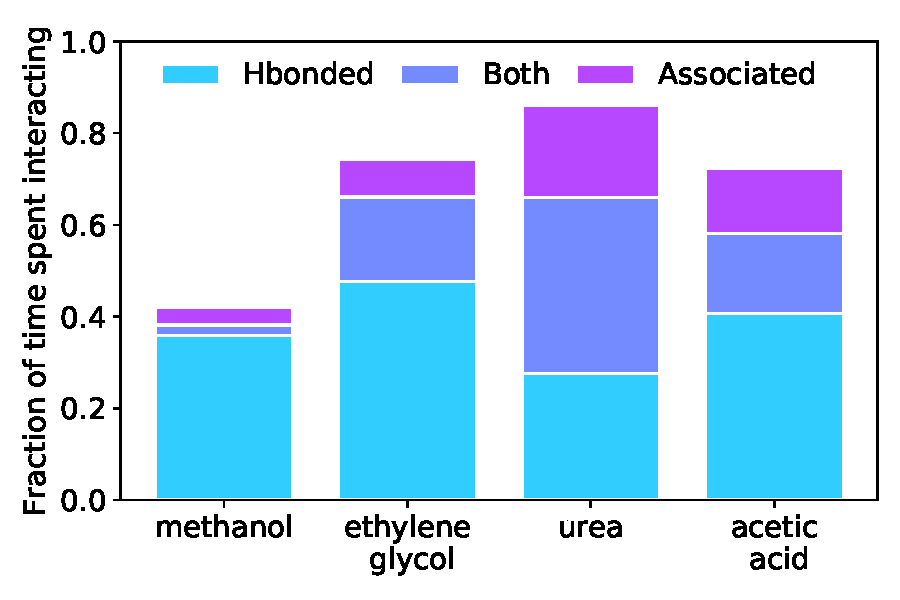
\includegraphics[width=\textwidth]{hbonds_assoc_summary.pdf}
  \caption{}\label{fig:hbonds_assoc_summary}
  \end{subfigure}
  \begin{subfigure}{0.45\textwidth}
  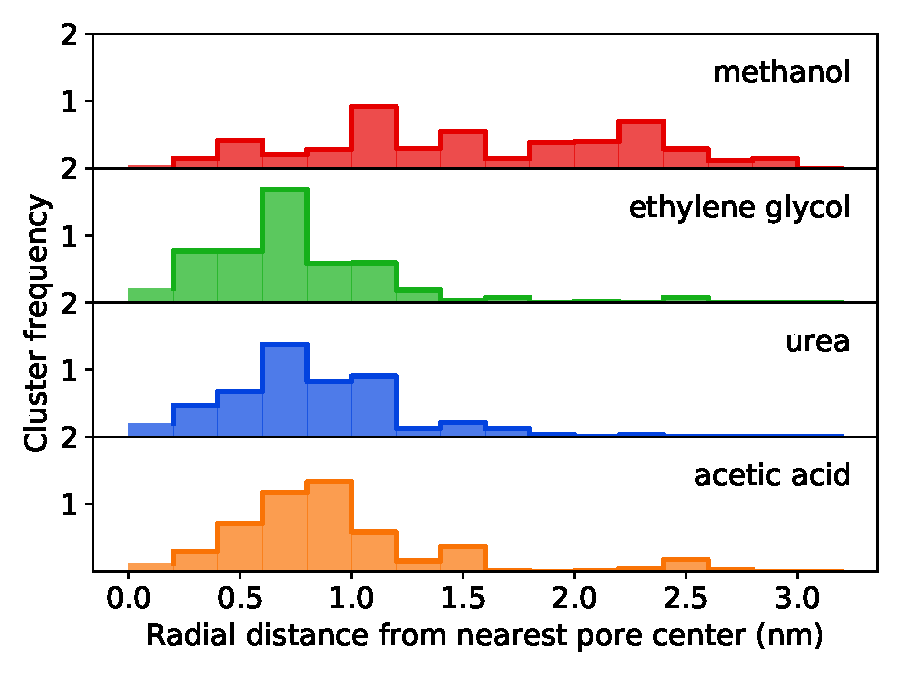
\includegraphics[width=\textwidth]{rdf_summary.pdf}
  \caption{}\label{fig:rdf_summary}
  \end{subfigure}
  \begin{subfigure}{0.45\textwidth}
  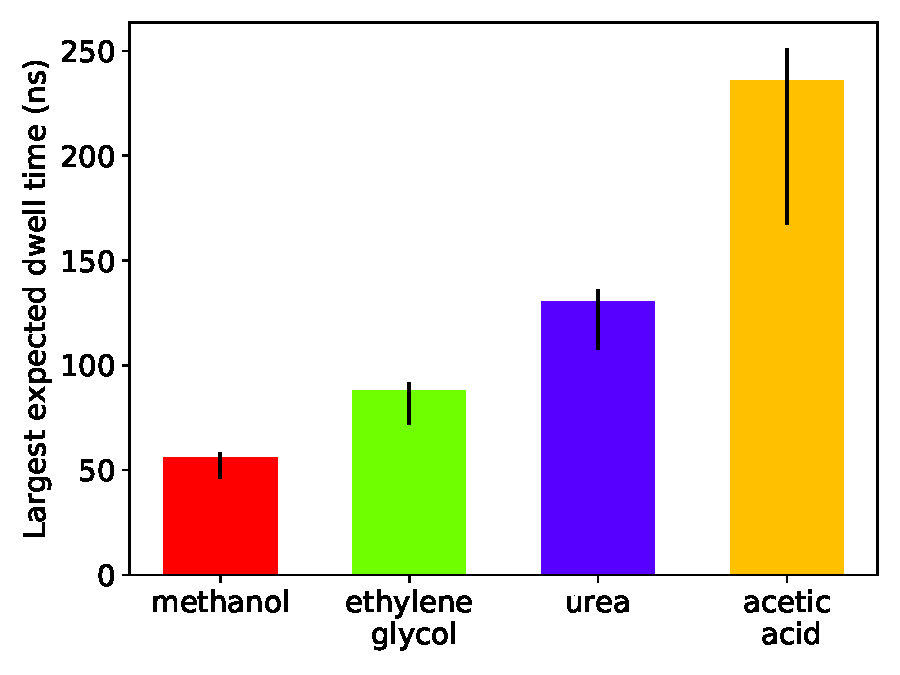
\includegraphics[width=\textwidth]{dwell_time_summary.pdf}
  \caption{}\label{fig:dwell_time_summary}
  \end{subfigure}
  \begin{subfigure}{0.45\textwidth}
  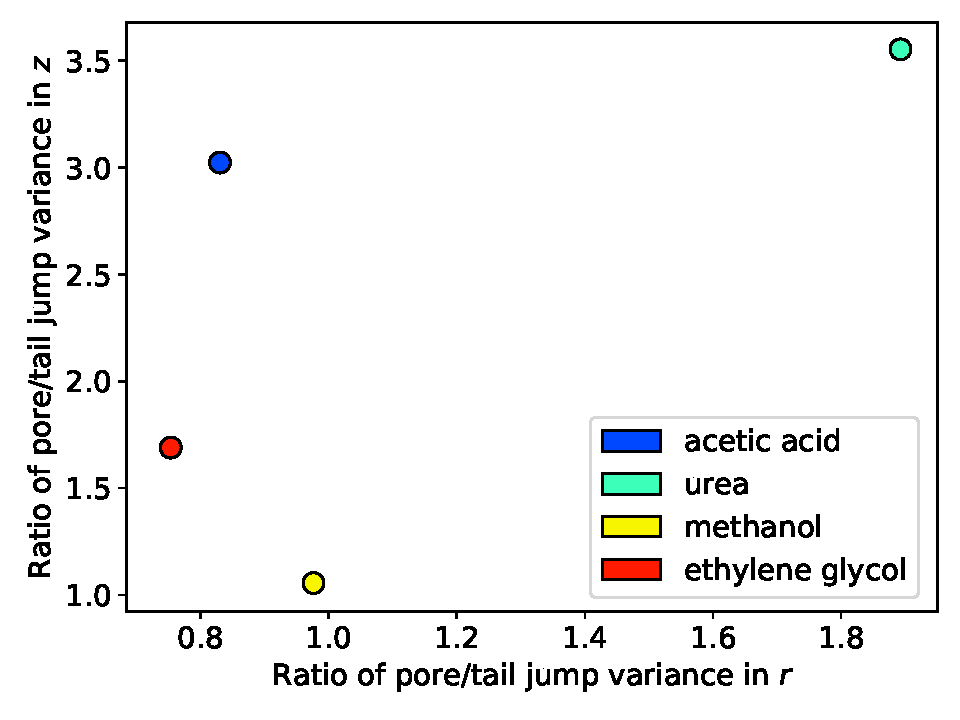
\includegraphics[width=\textwidth]{cov_summary.pdf}
  \caption{}\label{fig:cov_summary}
  \end{subfigure}
  %MRS7: is c) methanol?  I thought it wasn't associating with Na+ much.
  %BJC7: looks about 5 %, certainly less than the other. I could add
  % some discussion of this to previous section.
  %MRS: methanol yellow is hard to see in (b). Maybe add outlines to histogram?  I guess they are, increase alpha or something for yellow?
  %MRS: check consistency of capitalization in legend in (c) 
  \caption{(a) Solutes hydrogen bond and associate with sodium ions
  to different degrees. Sometimes, they participate in both interactions at
  once. The frequency at which solutes interact via either mechanism does
  not appear to be linearly related to the solute's mean squared displacement
  after a 1000 ns time lag. (b) We histogrammed the means of the clusters weighted
  by the number of fluctuation within that cluster. Most solutes spend the majority of
  their time close to the pore center. Only methanol has a significant peak
  beyond 1.5 nm from the pore center. (c) The trend in the maximum dwell time
  among prevalent states for each solute is inversely related to the
  solute's MSD. In some cases, non-prevalent states show very long dwell times,
  which may have a significant impact on solute MSD. (d) All solutes tend to
  take larger hops in the $z$ direction when they are in the pore versus in 
  the tails. All solutes except urea make slightly larger radial hops while 
  in the tails.
  %BJC6: I made this plot out of curiosity, not sure if I'll use it yet.
  }\label{fig:summaries}
  \end{figure}
  
  Hydrogen bonding and sodium ion association interactions are far more 
  common when solutes stay near the pore centers. In Figure~\ref{fig:rdf_summary},
  we plot the distribution of the radial means of each cluster weighted by 
  the time spent in that cluster. All solutes except methanol spend the 
  majority of their time near the pore centers (roughly defined as within 
  1.5 nm). As we showed earlier, methanol spends a significant portion of its
  time trapped in the dense tails.
  
  % BJC: we can probably use this to create a new definition of the pore and tail region.
  % and perhaps focus on transitions between them.
  Solute size likely has a large effect on their preferred radial location within
  the pores. The histograms in Figure~\ref{fig:rdf_summary} have a clear vacancy 
  between what one might consider the pore and tail region, most evident in methanol's 
  distribution of radial positions. The area between the head groups and the distal
  regions of the tails is dense and hydrophobic which creates a considerable energy 
  barrier to be overcome in order to transition to that region.
  %BJC: I wonder if there is a state which corresponds to the jump from pore to tail region. Might be hard to pick up.
  Methanol is the smallest solute in this study and therefore appears to 
  have the easiest time crossing into the tails.

  Despite their close proximity to the low density aqueous pore region, acetic
  acid, ethylene glycol and urea exhibit a range of trapping behavior.
  It is clear that the number of polar interactions is not directly
  related to solute MSD. Acetic acid participates in a similar number of 
  interactions relative to urea and ethylene glycol, but its MSD is considerably
  lower. For the purpose of this analysis, as in the previous section, we 
  defined states that appear in more than one third of the trajectories to
  be prevalent states. In Figure~\ref{fig:dwell_time_summary}, we plot the\
  longest dwell times exhibited by each solute among the prevalent states as 
  well as out of all the states. The state which exhibits the longest dwell
  times among all acetic acid states appears in 9 different trajectories, 
  making it a prevalent state, and occurs 0.9 nm from the pore center.
  Although urea possesses the state with the longest dwell time among the
  solutes studied, it occurs in the tail region with prevalent states having 
  much shorter dwell times. Ethylene glycol appears to be the least subject to
  trapping.

%  The combination of a carbonyl group, which binds strongly to sodium, and a 
%  hydroxyl group, which can form strong hydrogen bonds, makes acetic acid
%  particularly prone to trapping.
%  BJC6: more complicated than this. I will revisit.
  
  \section{Conclusion}
  
  We have shown that the IHMM can be used to automatically parameterize solute 
  time series with an unknown number of latent dynamical modes. Initially, we applied
  the algorithm to each trajectory independently. For each solute studied, this resulted
  in over 300 distinct states. By clustering the parameter sets we were able to reduce 
  the state space to 10\% of its original size by grouping states with similar VAR
  parameters.
  
  We coupled analysis of the clustered parameter sets with measurements of membrane 
  properties and solute-membrane interactions in order to gain a detailed understanding
  of the diverse sets behavior exhibited by solutes in these membranes. We showed how
  solute motion is influenced by hydrogen bonding, sodium ion association and local
  membrane density. These interactions have a direct impact on the size and
  correlation of sequential solute steps.
  
  Finally, we show how one can generate stochastic realizations of our model that
  can qualitatively and quantitatively reproduce the behavior of MD solute 
  trajectories. The realizations show the hopping and trapping behavior that is
  characteristic of polar solutes in this system. We can also use them to reproduce
  the solute MSDs measured from the MD trajectories. The low computational expense 
  of generating these stochastic trajectories allows one to project solute behavior
  on much longer timescales and thus predict experimentally-relevant macroscopic 
  transport properties like solute flux and selectivity.
  
  We showcase this modeling approach by example, but it is important to
  recognize the generality of this analysis, especially in the context of molecular
  simulations. Vector autogregressive models can describe a diverse set of behavior
  and so the IHMM may be suited to study many types motion, including those not 
  characterized by hopping and trapping. The IHMM is a powerful approach for 
  understanding particle motion as well as for generating inexpensive models
  which can give macroscopic insight.
  
  \section*{Supporting Information}

  Detailed explanations and expansions upon the results and procedures mentioned in
  the main text are described in the Supporting Information. 
  %This information is
  %available free of charge via the Internet at http://pubs.acs.org.

  \section*{Acknowledgments}

  This work was supported in part by the ACS Petroleum Research Fund
  grant \#59814-ND7 and the Graduate Assistance in Areas of National Need (GAANN) 
  fellowship which is funded by the U.S. Department of Education. 
  Molecular simulations were performed using the Extreme Science and
  Engineering Discovery Environment (XSEDE), which is supported by National
  Science Foundation grant number ACI-1548562. Specifically, it used the Bridges
  system, which is supported by NSF award number ACI-1445606, at the Pittsburgh
  Supercomputing Center (PSC). This work also utilized the RMACC Summit supercomputer,
  which is supported by the National Science Foundation (awards ACI-1532235 and
  ACI-1532236), the University of Colorado Boulder, and Colorado State
  University. The Summit supercomputer is a joint effort of the University of
  Colorado Boulder and Colorado State University.

  \clearpage

  \bibliographystyle{ieeetr}
  \bibliography{hdphmm}

  %\newpage

  %\section*{TOC Graphic}

\end{document}

% LocalWords:  BJC micropollutants Desalination permeability nanofiltration LLC
% LocalWords:  Amphiphilic nanostructures Lyotropic amphiphilic lyotropic MSDDM
% LocalWords:  solutes selectivities solute nanoscopic timescales MSDs MSD HMMs
% LocalWords:  nonparameteric Parrinello Rahman barostat rescale transitioning
% LocalWords:  al's HMM Dirichlet HDP DP Wishart TODO SI al MATLAB teh gael pdf
% LocalWords:  nonparametric bayesian solute's reparameterized intracluster ca
% LocalWords:  delocalize Luzar Chandler histogrammed interpolator methanol's
% LocalWords:  nanostructure carboxylate VMD nonidealities hbonds outlier GAANN
% LocalWords:  autogregressive PRF ACS XSEDE ACI IHMM nanoporous flowback evy
% LocalWords:  timescale subdiffusive coscia subdiffusion calderon GROMACS der
% LocalWords:  berendsen gromacs spoel hess emailed plateauing hmm ne gelman AR
% LocalWords:  walt numpy GCL URE ACH IMMM subsubsection modT convective vmd Na
% LocalWords:  scannable subsubcaptions errorbars uncharacteristicness facelift
% LocalWords:  PSC RMACC hdphmm TOC
